%!TEX root = 00_arbeit.tex

%---------------------------------------------------------------------------------
%% Theorie

\section{Neuronale Netze}
Um ein künstliches, computerbasiertes System dazu zu befähigen selbstständig zu Lernen, gilt es vorab folgendes zu klären: Einerseits muss zu einem gewissen Grad klar sein, wie das menschliche Gehirn aufgebaut ist und wie es lernt. Zum anderen muss dieses Wissen in eine Form gebracht werden, die ein Computer interpretieren und ausführen kann.

In diesem Abschnitt wird somit erklärt, wie biologische neuronale Netze funktionieren und welche Ableitungen und Rückschlüsse sich daraus für künstliche neuronale Netze ergeben. Im Nachgang werden verschiedene, aktuelle Konzepte vorgestellt, wie eine Überführung in ein mathematisches Modell konkret aussehen kann. Diese Konzepte werden einander gegenübergestellt und schlussendlich gruppiert und klassifiziert.


\subsection{Biologische Neuronale Netze}

Der menschliche Körper verfügt über eine Reihe von Sinnesorganen, über die er kontinuierlich Daten aufnimmt. Rezeptoren in unseren Augen nehmen beispielsweise visuelle Stimuli in Form von Lichtwellen auf, unsere Ohren akustische Signale in Form von Schallwellen. All diese Daten fließen in verschiedene Gehirnareale. Unser Gehirn besteht aus einer Menge an kleinen sowie großen anatomischen Strukturen und kann vereinfachend in vier Bereiche unterteilt werden (siehe \autoref{fig:Gehirn}). Das Großhirn (Telencephalon) ist hierbei für abstrakte Denkaufgaben zuständig. Unterhalb des Großhirns liegt das Kleinhirn (Cerebellum), welches die Motorik koordiniert und steuert. Daneben gibt es noch das Zwischenhirn (Diencephalon), das für die grundlegenden Körpervorgänge zuständig ist. Schließlich verbindet das Stammhirn (Truncus cerebri) das Gehirn mit dem Rückenmark und steuert die Körperreflexe.

\begin{figure}[!htb]
    \centering
        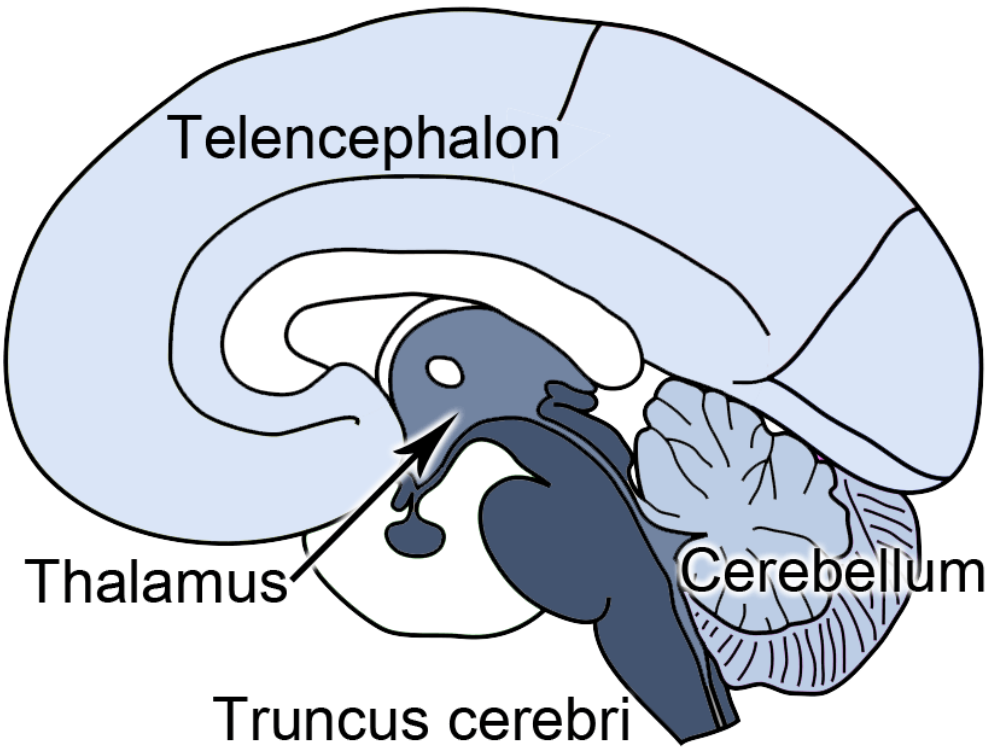
\includegraphics[width=0.5\textwidth]{Bilder/misc/Gehirn.png}
    \caption[Querschnitt des menschlichen Gehirns]{Querschnitt des menschlichen Gehirns mit den im Text genannten Arealen.\,\protect\footnotemark{}}
    \label{fig:Gehirn}
\end{figure}
\addtocounter{footnote}{-1}     % -1 mal die Gesamtanzahl an Fußnoten in der wrapfigure
\addtocounter{Hfootnote}{-1}    % -1 times total number of footnote(mark)s in the wrapfigure
\wrapfigfoot\footnotetext{\autoref{fig:Gehirn} wurde aus \citet[17]{dkriesel07} übernommen.}

In all diesen Bereichen werden die gesammelten Daten der Sinnesorgane zu Informationen verarbeitet. Dies wird durch Milliarden sehr ähnlicher Zellen bewerkstelligt, welche miteinander kommunizieren. Diese Zellen werden als Neuronen bezeichnet. Der Aufbau und die Verbindung zweier Neuronen ist in \autoref{fig:Neuronen} dargestellt. Betrachtet wird nun der Weg, den die elektrischen Signale in einem Neuron nehmen.

\begin{figure}[!htb]
    \centering
        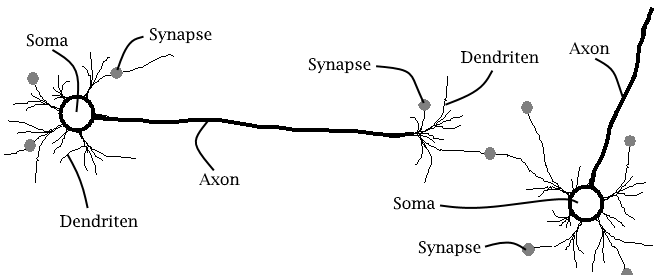
\includegraphics[width=0.8\textwidth]{Bilder/misc/Neuronen.png}
    \caption[Verbindung zweier biologischer Neuronen]{Verbindung zweier Neuronen in einem biologischen neuronalen Netz.\,\protect\footnotemark{}}
    \label{fig:Neuronen}
\end{figure}
\addtocounter{footnote}{-1}     % -1 mal die Gesamtanzahl an Fußnoten in der wrapfigure
\addtocounter{Hfootnote}{-1}    % -1 times total number of footnote(mark)s in the wrapfigure
\wrapfigfoot\footnotetext{\autoref{fig:Neuronen} wurde aus \citet[2]{sen_an} übersetzt und angepasst.}

Daten aus Sensorzellen, wie zum Beispiel den Fotorezeptoren in unseren Augen, werden über elektrische Impulse von einem Neuron zum anderen weitergegeben. Die Übertragung des Impulses findet an den sogenannten Synapsen statt. Die Synapsen liegen meistens auf den Dendriten, welche sich baumartig vom Soma (dem Zellkern des Neurons) ausbreiten und für die Aufnahme der elektrischen Signale verschiedener Quellen zuständig sind. Die so im Soma eintreffenden Signale wirken entweder anregend oder abschwächend. Das Soma kumuliert die eintreffenden Signale auf. Ab einem bestimmten Wert, der als Schwellwert bezeichnet wird, schickt das Soma über das Axon seinerseits einen elektrischen Impuls. Das Axon leitet den Impuls wiederum über Synapsen an die Dendriten eines nachfolgenden Neurons. Abstrakt kann ein Neuron somit als Schalter mit einem Ein- und Ausgang betrachtet werden, welcher Daten weiterreicht.\,\citef[15 ff]{dkriesel07} Die Verbindungen aus mehreren Neuronen werden als neuronales Netz bezeichnet und so bilden verschiedene neuronale Netze verschiedene Areale in unserem Gehirn. 

% Das Gehirn verfügt bereits zur Geburt über den größten Teil seiner Neurone. Allerdings sind die Verbindungen zwischen ihnen noch nicht stark ausgeprägt. Dies geschieht vereinfacht gesagt durch Lernen. Je öfter eine Lernerfahrung gemacht wird, desto stärker werden die Verbindungen der beteiligten Neuronen und desto stabiler werden sie. Außerdem speichert das menschliche Gehirn Informationen besser ab, wenn mehrere Neuronen ihren Input beigetragen haben.\farbig{Quelle?}

\subsection{Künstliche Neuronale Netze}\label{sec:einf_neuro}



%\subsection{Globaler Überblick über Neuronale Netze}
%\farbig{[Erklärung der neuronalen Netze... vielfältige Anwendungsgebiete... Hier erforderlich Netze zur Zeitreihenvorhersage]}
%\setlength{\intextsep}{0pt}%

%\begin{wrapfigure}{r}{0.5\textwidth}
%    \centering
%        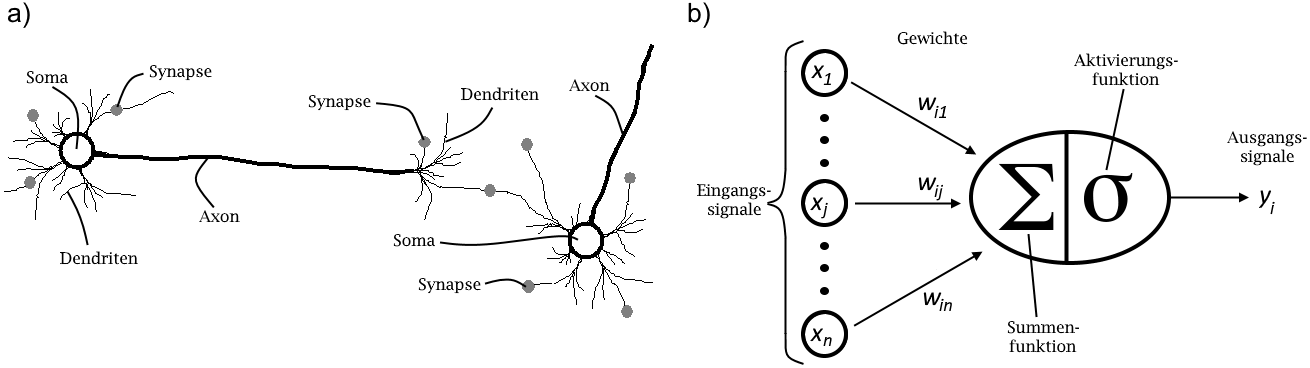
\includegraphics[width=0.5\textwidth]{Bilder/BNN_ANN.png}
%    \caption{Gegenüberstellung eines Ausschnittes aus einem biologischen neuronalen Netz a)\protect\footnotemark{} und einem künstlichen neuronalen Netz b).}
%    \label{fig:BNN_ANN}
%\end{wrapfigure}


%\citet[\pno~2~ff.]{sen_an}

Künstliche neuronale Netze sind augenblicklich eine Disziplin der Computerbasierten Intelligenz (engl.: computional intelligence)~(\gls{CI}), welches wiederum einen Teilbereich der Künstlichen Intelligenz (engl.: artificial intelligence)~(\gls{AI}) darstellt. Die CI fasst verschiedene, von der Natur inspirierte Berechnungsmethoden zusammen. Neben den künstlichen neuronalen Netzen (engl. artificial neural networks)~(\gls{NN}) existieren weitere Methoden der CI Fuzzy-Systeme~(\gls{FS}), Evolutionäre Algorithmen~(\gls{EA}), Schwarmintelligenz~(\gls{SI}) und Künstliche \hbox{Immunsysteme~(\gls{AIS})}.\,\citef[11 ff]{Kroll16} Obwohl sich diese Arbeit wesentlich mit NN beschäftigen wird, wird an dieser Stelle auf weitere CI-Methoden hingewiesen, da in der Literatur hybride CI-Systeme bekannt sind und auch genutzt werden.

Ein künstliches neuronales Netz ist ein mathematisches Konstrukt. Es bildet ein informationsverarbeitendes System, welches aus einer Vielzahl einfacher Einheiten besteht. Entstanden ist es Anfang der 40er Jahre des letzten Jahrhunderts\,\citef[A1.1:1]{Fiesler96} aus der Untersuchung von biologischen Abläufen im Nervensystem, wie sie im vorangegangenen Abschnitt erläutert wurden. 

\begin{figure}[!htb]
    \centering
        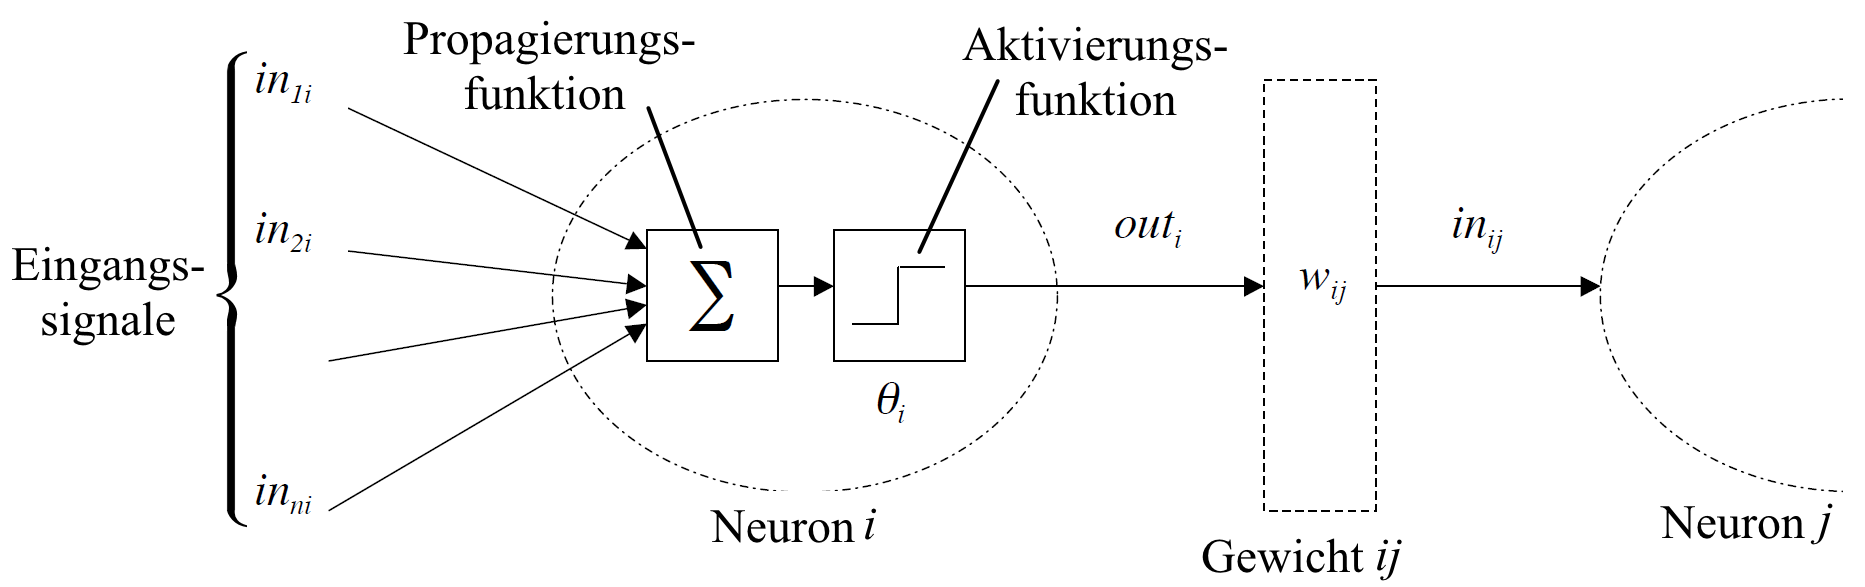
\includegraphics[width=1\textwidth]{Bilder/misc/kuenstliches_neuron.png}
    \caption[Künstliches Neuron (Perceptron)]{Ausschnitt eines künstlichen neuronalen Netzes mit dem Fokus auf ein Neuron.\,\protect\footnotemark{}}
    \label{fig:KNN}
\end{figure}

\addtocounter{footnote}{-1}     % -1 mal die Gesamtanzahl an Fußnoten in der wrapfigure
\addtocounter{Hfootnote}{-1}    % -1 times total number of footnote(mark)s in the wrapfigure
\wrapfigfoot\footnotetext{Die \autoref{fig:KNN} wurde aus \citet[2]{Bullinaria2015} übersetzt und angepasst.}


Diese einfachen Einheiten werden nach ihren biologischen Vorbildern ebenfalls als Neuronen bezeichnet. In Anlehnung an die Funktion des biologischen Neurons wurde die Funktion des künstlichen Neurons, dargestellt in \autoref{fig:KNN}, folgendermaßen beschrieben:

Die in einem Neuron eintreffenden Signale werden zunächst mit der Propagierungsfunktion verarbeitet. Oftmals ist die Propagierungsfunktion eine Summe der verschiedenen Eingänge. Somit werden die eintreffenden Signale zunächst aufsummiert. Mit Hilfe der Aktivierungsfunktion wird anschließend untersucht, ob der zuvor summierte Wert eine Aktivität des künstlichen Neurons hervorrufen kann. Ist dies der Fall, so sendet das Neuron den Ausgabewert der Aktivierungsfunktion an das nachfolgende Neuron. Die Verbingung von einem zum anderen Neuron findet in dem biologischen Vorbild über die Synapse statt. Mathematisch ist dies durch ein Gewicht repräsentiert. Hierdurch wird die Stärke der Verbindung zwischen zwei Neuronen ausgedrückt. Der grundlegende Aufbau folgt also dem des biologischen Pendants: Somit können die Signalkanäle des künstlichen Neurons als Dendriten, die Propagierungs- sowie Aktivierungsfunktion als Soma, die Ausgabe als Axon und die Gewichtung als Synapse des biologischen Neurons betrachtet werden.

Aus diesem Grundgerüst lassen sich nun Netze zusammensetzen. Entscheidend ist hierbei die Verbindung zwischen den Neuronen. Hier wird das Wissen in Form der Gewichte gebildet und gespeichert. Ein neuronales Netz lernt, indem diese Gewichte modifiziert werden. Je größer der Wert des Gewichts ist, desto stärker ist die Verbindung. In Analogie zu biologischen neuronalen Netzen haben positive Gewichte einen erregenden Einfluss auf das nachfolgende Neuron, negative Gewichte haben hingegen einen hemmenden Einfluss.\,\citef[17]{bio_neuron}

Wie die Gewichte im Detail angepasst und verändert werden, wird durch den sogenannten Lernalgorithmus beschrieben. Wie auch beim Menschen muss sich ein künstliches neuronales Netz entwickeln. Dies geschieht in der Regel in einer Trainings- und Testphase. Auf Basis eines zur Verfügung gestellten Lernmaterials (beim künstlichen Netz in Form von Eingabe-Daten) wird ein Lernalgorithmus angewandt. Im Ergebnis kommt das Netz schlussendlich zu einer stabilen Gewichtsverteilung, die das dann erlangte Wissen repräsentiert.



\subsection{Charakterisierung künstlicher neuronaler Netze}\label{sec:char}

Neuronale Netze können auf verschiedene Arten und Weisen konzipiert werden. Für jedes Element des eben beschriebenen Aufbaus gibt es verschiedene Ausprägungen, die wiederum unterschiedlich miteinander verknüpft und zusammengesetzt werden können. Es gibt also nicht das eine eingesetzte Neuron und nicht das eine neuronale Netz, sondern viele unterschiedliche, die teilweise spezielle Anwendungsgebiete finden.

Im Allgemeinen können Neuronale Netze hinsichtlich folgender Einordnungen charakterisiert werden:\,\citef[7 ff]{characterisation_4}
\begin{itemize}
\item[\textbf{$\bullet$}] Art des Neurons

\item[\textbf{$\bullet$}] Topologie und Verbindungsarchitektur des Netzes

\item[\textbf{$\bullet$}] Eingesetzter Lernalgorithmus
\end{itemize}

\subsubsection{Unterscheidung nach Art des Neurons}

Das zurzeit prominenteste künstliche Neuron, welches in \autoref{fig:KNN} dargestellt ist, wird nach \citet{perceptron_ros58} als Perceptron bezeichnet. So summiert es zunächst die gewichteten Eingangsinformationen mit der Propagierungsfunktion, anschließend wird die gewichtete Summe über die Aktivierungsfunktion als Ausgang an das nächste Neuron übergeben. Die eingesetzte Aktivierungsfunktion kann dabei variieren. In \autoref{fig:funktion} sind klassische Aktivierungsfunktionen dargestellt. Die Aktivierungsfunktion beschreibt den Zusammenhang zwischen dem Eingangssignal und dem Aktivierungslevel des Neurons. Die Funktion reglementiert somit, ob ein gewisser Schwellwert erreicht werden muss, um das Neuron zu aktivieren und wenn ja, wie dieser Zusammenhang mathematisch ausgedrückt werden kann. Die Heavisidefunktion fungiert beispielsweise wie eine Art Schalter, der nur zwei Zustände kennt. Lineare Schwellwertfunktionen können eingesetzt werden, wenn die zu untersuchenden Daten linear separierbar sind. Sigmoide Aktivierungsfunktionen, wie die logistische Funktion und der Tangens Hyperbolicus nähern sich dem biologischen Vorbild des Axons am weitesten an und bieten damit in gewissen Anwendungsgebieten Vorteile in Bezug auf Plausibilität, Differenzierbarkeit und Begrenzung des Aktivitätslevels. Sowohl die Heavisidefunktion, als auch die lineare Schwellwertfunktion und der Tangens Hyperbolicus können sowohl bipolar (Wertebereich [-1,1]), aber auch unipolar (Wertebereich [0,1]) verwendet werden. Die logistische Funktion weist zwar nur einen Wertebereich von [0,1] auf, aber durch den Temperaturfaktor kann sie an die Heavisidefunktion angenähert werden und hat dann den Vorteil der Differenzierbarkeit .\,\footnote{Vgl. \citet[5]{neuralnet_intro} und \citet[39 f]{dkriesel07}.} Die Differenzierbarkeit ist für einige Lernalgorithmen, auf die in \autoref{sec:algorithm} näher eingegangen wird, eine wichtige Eigenschaft, da dort die Aktivierungsfunktion abgeleitet werden muss.

\begin{figure}[!htb]
    \centering
    %\WarningsOff*
    
    \includestandalone[mode=image|tex]{Bilder/misc/Aktivierungsfunktionnen}
    %\documentclass[tikz,border=0pt]{standalone}%
\usepackage{tikz-cd}
%\usepackage{silence}
\usetikzlibrary{arrows}
%\ErrorsOff*

\begin{document}
        %---------------------------------------------------------------
        %% Heaviside
        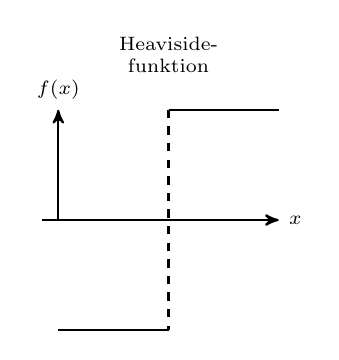
\begin{tikzpicture}[scale=.7,font=\scriptsize,thick,>=stealth']
            \coordinate (O) at (0,0);
            % horizontal axis
            \draw[->] (-0.3,0) -- (4,0) coordinate[label = {right:$x$}] (xmax);
            % vertical axis
            \draw[->] (0,0) -- (0,2) coordinate[label = {above:$f(x)$}] (ymax);
  
            \node[align=center] at (2,3) {Heaviside-\\funktion};
  
            \draw (2,2) -- (4,2);
            \draw (2,-2) -- (0,-2);
            \draw[dashed] (2,2) -- (2,-2);
        \end{tikzpicture}
        %---------------------------------------------------------------
        %% lineare Schwellwertfunktion
        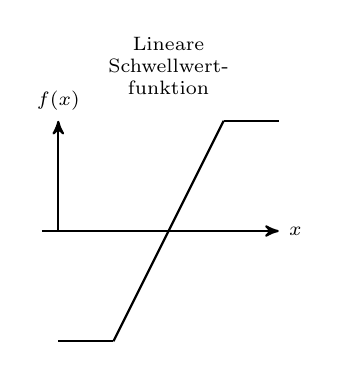
\begin{tikzpicture}[scale=.7,font=\scriptsize,thick,>=stealth']
            \coordinate (O) at (0,0);
            % horizontal axis
            \draw[->] (-0.3,0) -- (4,0) coordinate[label = {right:$x$}] (xmax);
            % vertical axis
            \draw[->] (0,0) -- (0,2) coordinate[label = {above:$f(x)$}] (ymax);
  
            \node[align=center] at (2,3) {Lineare\\Schwellwert-\\funktion};
  
            \draw (3,2) -- (4,2);
            \draw (1,-2) -- (0,-2);
            \draw (1,-2) -- (3,2);
        \end{tikzpicture}
        %---------------------------------------------------------------
        %% Fermifunktion
        \begin{tikzpicture}[scale=.7,font=\scriptsize,thick,>=stealth']
            \draw[white] (1,-2) -- (3,2);
            
            \draw[scale=.5,domain=-4:4,smooth,variable=\x,lightgray]      plot ({\x+4},{4*(1/(exp(-\x/.2)+1))});
            \draw[scale=.5,domain=-4:4,smooth,variable=\x,lightgray]      plot ({\x+4},{4*(1/(exp(-\x/.5)+1))});
            \draw[scale=.5,domain=-4:4,smooth,variable=\x,black]          plot ({\x+4},{4*(1/(exp(-\x/.8)+1))});
            % horizontal axis
            \draw[->] (-0.3,0) -- (4,0) coordinate[label = {right:$x$}] (xmax);
            % vertical axis
            \draw[->] (0,0) -- (0,2) coordinate[label = {above:$f(x)$}] (ymax);
            \node[align=center] at (2,3) {Logistische\\Funktion};
        \end{tikzpicture}
        %---------------------------------------------------------------
        %% Tangens Hyperbolicus
        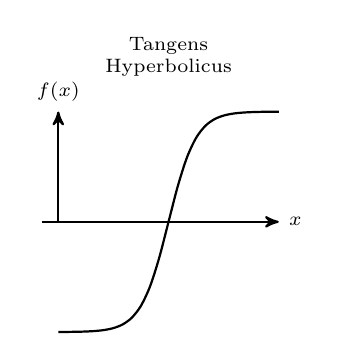
\begin{tikzpicture}[scale=.7,font=\scriptsize,thick,>=stealth']
            \coordinate (O) at (0,0);
            % horizontal axis
            \draw[->] (-0.3,0) -- (4,0) coordinate[label = {right:$x$}] (xmax);
            % vertical axis
            \draw[->] (0,0) -- (0,2) coordinate[label = {above:$f(x)$}] (ymax);
            \node[align=center] at (2,3) {Tangens\\Hyperbolicus};
            \draw[scale=0.5,domain=-4:4,smooth,variable=\x,black] plot ({\x+4},{4*tanh(\x)});
        \end{tikzpicture}
\end{document}
    \caption[Typische Aktivierungsfunktionen]{Typische Funktionen die als Aktivierungsfunktion angewendet werden.\,\protect\footnotemark{}}
    \label{fig:funktion}
\end{figure}
\addtocounter{footnote}{-1}     % -1 mal die Gesamtanzahl an Fußnoten in der wrapfigure
\addtocounter{Hfootnote}{-1}    % -1 times total number of footnote(mark)s in the wrapfigure
\wrapfigfoot\footnotetext{\autoref{fig:funktion} wurde in Anlehnung an \citet[5]{neuralnet_intro} Figure 1.5 erstellt.}

Das Perceptron ist, wie eingangs erwähnt, nicht die einzige denkbare mathematische Repräsentation eines Neurons. Im später vorgestellten Hopfield-Netzwerk wird das Neuron als ein Teilchen beschrieben, welches sich in einem Magnetfeld ausrichtet.\,\citef[135]{dkriesel07} Ein eher exotischer Vertreter ist darüber hinaus das Fuzzy-Neuron\,\citef[276 ff]{fuzzyneuron}, welches nach der Aktivierung mehrere mögliche Zustände einnehmen kann und seine Anwendung in der Mustererkennung findet. 

\newpage

\subsubsection{Unterscheidung nach Art der Topologie bzw. der Verbindungsarchitektur}

Die Topologie beschreibt, wie Neuronen in einem Netzwerk verbunden sind. Ein Unterscheidungskriterium ist dabei die Assoziativität:
\begin{itemize}
\item[\textbf{$\bullet$}] Bei autoassoziativen Netzen fungieren die Eingangsneurone gleichzeitig als Ausgangsneurone.

\item[\textbf{$\bullet$}] Heteroassoziative Netze unterscheiden hingegen zwischen Eingangs- und Ausgangsneuronen.
\end{itemize}

Zusätzlich wird unterschieden wie die Verbindungen unter den einzelnen Neuronen realisiert sind. Neuronale Netze können sich aus verschiedenen Schichten zusammensetzen. Die Anzahl der Schichten kann dabei ebenfalls variieren. Schichten können beispielsweise dazu dienen Daten zwischen der Eingangs- und Ausgangsschicht weiter zu verarbeiten. Die Weitergabe von Daten, über verschiedene Schichten hinweg, kann dabei grundsätzlich auf zwei verschiedenen Arten erfolgen:\,\citef[42 ff]{dkriesel07}

\begin{itemize}
\item[\textbf{$\circ$}] Feed-Forward: Hierbei ist eine Schicht nur mit der jeweils nächsten Schicht verbunden, sodass die Informationen von Schicht zu Schicht vorwärtsgerichtet weitergegeben wird.

\item[\textbf{$\circ$}] Recurrent (Feed-Back): In der deutschsprachigen Literatur als rückgekoppelte oder rekurrente Netze bezeichnet, beeinflussen sich die Schichten dieser Netzwerke gegenseitig. Die Neuronen dieser Netzwerke besitzen eine Verbindung entweder zu sich selbst (direkte Rückkoppelung), zu den Neuronen der vorhergehenden Schicht (indirekte Rückkopplung), zu den Neuronen der gleichen Schicht (laterale Rückkopplung) oder vollverknüpfte Netze (Verbindungen zwischen allen Neuronen ausgenommen der direkten Rückkopplung). Durch die Rückkopplung besitzen diese Netzwerke ein \glqq Gedächtnis\grqq , da der vorherige Zustand in die Auswertung der aktuellen Eingangsinformation mit einfließt.
\end{itemize}



\subsubsection{Unterscheidung nach dem Lernalgorithmus }
Wie eingangs erwähnt, lernt das neuronale Netz, indem es Trainingsdaten mithilfe eines Lernalgorithmus verarbeitet. Wobei ein Netzwerk mit unterschiedlichen Lernalgorithmen trainiert werden kann. Die derzeitig benutzten Algorithmen lassen sich in drei Gruppen unterteilen: 
\begin{itemize}
\item[\textbf{$\bullet$}] Supervised learning (überwachtes Lernen): Die Trainingsbeispiele bestehen hierbei aus einer Menge an Eingangsinformationen und den dazugehörigen Ausgangsinformationen. Das Ziel ist es, die Differenz zwischen der tatsächlichen Ausgabe des Netzwerks und den vorliegenden Ausgangsinformationen zu minimieren. Die Gewichte dieses Netzes werden somit anhand des überprüfbaren Outputs modifiziert.


\item[\textbf{$\bullet$}] Reinforcement learning (bestärkendes Lernen): Plakativ kann diese Lernmethode als Zuckerbrot und Peitsche bezeichnet werden bzw. lernen durch Belohnung und Bestrafung. Hierbei werden die Eingangsinformationen zur Verfügung gestellt und die Ausgabe des Netzwerkes wird anhand einer Belohnungsfunktion bewertet. Wird die Ausgabe als gut/schlecht angesehen, so werden die zugehörigen Verbindungen gestärkt beziehungsweise geschwächt .\,\footnote{Vgl. \citet[201]{dkriesel07} und \citet[A2.3:5]{Fiesler96}.}


\item[\textbf{$\bullet$}] Unsupervised learning (unüberwachtes Lernen): Wird auch als selbstorganisiertes (self organized) Lernen bezeichnet. Die Trainingsbeispiele bestehen hierbei nur aus Eingansinformationen. Das Netzwerk versucht aus den Eingansinformationen selbstständig Ähnlichkeiten zu erkennen. Unüberwachte Lernmethoden werden noch unterteilt in konkurrierendes (competitive) und nicht konkurrierendes (noncompetitive) Lernverfahren. Der Unterschied besteht darin, dass bei dem konkurrierenden Verfahren in einem Netzwerk einzelne Gruppen von Neuronen um die Aktivität konkurrieren.\,\citef[B3.3:5]{Fiesler96}

\end{itemize}

Zusätzlich unterscheidet man unter allen drei Lernmethoden zwei Lernarten:\,\citef[A2.3:3]{Fiesler96}

\begin{itemize}
\item[\textbf{$\circ$}] Beim Off-line learning, auch Batch-Trainingsverfahren genannt, wird die Netzwerkausgabe zunächst nach einer Menge von Eingangsinformationen ausgewertet und anschließend werden die Gewichte angepasst.


\item[\textbf{$\circ$}] Beim on-line learning werden die Gewichte nach jeder einzelnen Beobachtung der gesamten Eingangsinformationen angepasst.

\end{itemize}


\subsection{Vorstellung einiger Modelle}\label{sec:ANN-Modelle}
Nachdem im vorherigen Unterabschnitt die Charakterisierung der NN beleuchtet wurde, wird in diesem Unterabschnitt die Funktionsweise einiger künstlicher neuronaler Netze erläutert, wobei die hier vorgestellten Netzwerke einem informativen Überblick über die Vielfalt an künstlichen neuronalen Netzen dienen.

%\newpage

\subsubsection{Perceptrons (SLP)/(MLP)}
Die Einzelschichtperceptrons (single layer perceptrons)~(\gls{SLP}) und Mehrschichtperceptrons (multi layer perceptrons)~(\gls{MLP}) zählen zu den Feed-Forward Netzen, die überwacht trainiert werden. Bei den Einzelschichtperceptrons werden die zuvor in \autoref{sec:einf_neuro} beschriebenen Perceptrons zu einem Netzwerk zusammengeschlossen. \autoref{fig:SLP} zeigt ein SLP mit fünf Eingabeneuronen $i$ und zwei Ausgabeneuronen $\Omega$.



\begin{figure}[!htb]
    \centering
        %---------------------------------------------------------------
        %% SLP
        %-----------------------------------------
                %---------------------------------------------------------------
        %% SLP
        %-----------------------------------------
        %% linkes Bild
        \begin{tikzpicture}[>=stealth', node distance=\layersep cm, shorten >=1pt]
        \def\layersep{2}            % vertikal distance between the layers
        \def\neuronsep{1.5}         % Horizontal distance between neurons
        \def\dlsize{1.5}            % distance between node and layer lable
        \def\inout{\layersep*.65}   % Size of in- and output-arrow
        \def\siz{.8}                % neuronsize
        \def\y{3}                   % Start of the most upper layer
        \def\ni{5}                  % Amount of input neurons
        \def\no{2}                  % Amount of output neurons
        \tikzstyle{neuron}=[circle,draw=black,minimum size=\siz cm,inner sep=2pt]
        \tikzstyle{annot} = [text width=5em, text centered]
        \tikzset{fontscale/.style = {font={\fontsize{#1pt}{#1pt}\selectfont}}}
        \newcommand{\neurono}[2][]{
            \node[neuron,circle split,inner sep=2pt] (#1) at (#2)
                    {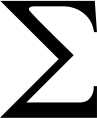
\includegraphics[width=0.225cm]{Bilder/Sigma.png} \nodepart{lower} 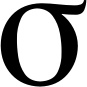
\includegraphics[width=0.225cm]{Bilder/sigma.png}};
        }

        % Draw the left input layer nodes
            \foreach \name / \xn in {1,...,\ni}{
            % This is the same as writing \foreach \name / \y in {1/1,2/2,3/3,4/4}
                \node[neuron,fontscale=15] (Il-\name) at (\xn*\neuronsep-\neuronsep,\y) {$i_{\xn}$};
                \node[above of=Il-\name, node distance=\inout cm] (Inl-\name) {};
                \draw [->,arrows={-Stealth[length=7pt]},densely dotted] (Inl-\name) edge (Il-\name);
            }
        % Draw the output layer node
            \foreach \name / \xn in {1,...,\no}{
                \node[neuron,fontscale=15] (Ol-\xn) at ({(\ni-1)*\neuronsep/2-\neuronsep/2*(\no-1)+(\xn-1)*\neuronsep},\y-\layersep) {$\Omega_{\xn}$};
                \node[node distance=\inout cm, below of=Ol-\xn] (Onl) {};
                \draw [->,arrows={-Stealth[length=7pt]},densely dotted] (Ol-\xn) edge (Onl);
        % Connect every node in the input layer with the output layer
            \foreach \source in {1,...,\ni}
                \draw [->,arrows={-Stealth[length=7pt]}] (Il-\source) edge (Ol-\xn);
                }
        % Annotate the layers
                \node[annot,right of=Il-\ni, node distance=\dlsize cm] (il) {\textbf{Eingabe- schicht}};
                \node[annot,below of=il] {\textbf{Ausgabe- schicht}};
        %-----------------------------------------
        %% rechtes Bild
            \tikzset{
                ident/.pic={
                \draw[semithick] (-\siz/4,-\siz/4) -- (\siz/4,\siz/4);
            }}
        % Draw the right input layer nodes
                \node[xshift=\dlsize cm] (Ir) at (il) {};
            \foreach \name / \xn in {1,...,\ni}{
        % This is the same as writing \foreach \name / \y in {1/1,2/2,3/3,4/4}
                \node[neuron] (Ir-\name) at ($(Ir)+(\xn*\neuronsep-\neuronsep,0)$) {};
                \node[above of=Ir-\name, node distance=\inout cm] (Inr-\name) {};
                \pic at (Ir-\name) {ident};
                \draw [->,arrows={-Stealth[length=7pt]},densely dotted] (Inr-\name) edge (Ir-\name);
            } 
        % Draw the output layer node
            \foreach \name / \xn in {1,...,\no}{
                \neurono[Or-\xn]{$(Ir)+({(\ni-1)*\neuronsep/2-\neuronsep/2*(\no-1)+(\xn-1)*\neuronsep},-\layersep)$}

                \node[node distance=\inout cm, below of=Or-\xn] (Onr) {};
                
                \draw [->,arrows={-Stealth[length=7pt]},densely dotted] (Or-\xn) edge (Onr);
                
        % Connect every node in the input layer with the output layer
            \foreach \source in {1,...,\ni}
                \draw [->,arrows={-Stealth[length=7pt]},every node/.style={fill=white,inner sep=1pt,fontscale=7}] 
                (Ir-\source) edge  (Or-\xn) 
                node at ($(Ir-\source)!.3+.18*(\xn-1)!(Or-\xn)$) {$w_{\source,\xn}$};
            }
\end{tikzpicture}
    \caption[Darstellung eines SLP]{SLP mit fünf Eingabeneuronen $i$ und zwei Ausgabeneuron $\Omega$ auf der linken Seite. Die rechte Seite zeigt das gleiche Netzwerk mit den zugehörigen neuronalen Aufgaben und Gewichten.\,\protect\footnotemark{}}
    \label{fig:SLP}
\end{figure}
\addtocounter{footnote}{-1}     %  -1 mal die Gesamtanzahl an Fußnoten in der wrapfigure
\addtocounter{Hfootnote}{-1}    % -1 times total number of footnote(mark)s in the wrapfigure
\wrapfigfoot\footnotetext{Die linke Darstellung des SLP in \autoref{fig:SLP} wurde der Abbildung 5.3 aus \citet[77]{dkriesel07} nachempfunden.}

In der Literatur gibt es keine Konvention in der Hinsicht, ob die Eingabeneuronen $i$, welche als Identität dienen (in \autoref{fig:SLP} dargestellt als \inlineneuron[i]{0.7}) und Informationen nur weitergeben, auch als Schicht zählen. Wenn die Eingabeneuronen nicht hinzugezählt werden, so wird nur das datenverarbeitende Neuron \inlineneuron[per]{0.7} als Perceptron bezeichnet. Werden die Eingabeneuronen auch als Schicht gezählt, so wird das sich so ergebende neuronale Netz aus Eingabe- und Verarbeitungsschicht ebenfalls als Perceptron bezeichnet. In dieser Arbeit wird die Eingabeschicht mitgezählt. So besteht das SLP aus einer Schicht Eingabeneuronen und mindestens einem Ausgabeneuron. Beide Schichten sind verbunden über \underline{eine} Ebene trainierbarer Gewichte $\text{\textit{w}}$. Das SLP ist unter anderem in der Lage, logische Funktionen wie AND- und OR-Funktion zu erlernen. Es ist aber auf linear separierbare Daten beschränkt, sodass die XOR-Funktion (siehe Anhang~\ref{sec:XOR}) mit einem SLP nicht mehr realisiert werden kann. Da die logischen Funktionen als Grundbausteine der heutigen Informationsverarbeitung dienen, folgt aus der vorherigen Erläuterung, dass kompliziertere Funktionen mit einem SLP ebenfalls nicht realisiert werden können.
Um das SLP zu trainieren, gibt es mehrere Lernalgorithmen. Als Beispiele werden hier der Perceptron-Lernalgorithmus\,\citef[78]{dkriesel07} und die Deltaregel (siehe Anhang~\ref{sec:deltaregel}) genannt, auf die im Anhang~\ref{sec:deltaregel} näher eingegangen wird. Letztere Methode hat im Vergleich zur ersteren den Vorteil, dass sie nicht nur auf binäre Aktivirungsfunktionen beschränkt ist und somit auch kontinuierliche Werte verarbeiten kann.\,\citef[76 ff]{dkriesel07}
%\\

\begin{figure}[!htb]
    \centering
    %---------------------------------------------------------------
        %% MLP
        %-----------------------------------------
            %---------------------------------------------------------------
        %% MLP
        %-----------------------------------------
        %% linkes Bild
\begin{tikzpicture}[>=stealth', node distance=\layersep cm, shorten >=1pt]
        \def\layersep{1.8}            % vertikal distance between the layers
        \def\neuronsep{1.8}         % Horizontal distance between neurons
        \def\dlsize{2}            % distance between node and layer lable
        \def\inout{\layersep*.65}   % Size of in- and output-arrow
        \def\siz{.8}                % neuronsize
        \def\y{5}                   % Start of the most upper layer
        \def\ni{3}                  % Amount of input neurons
        \def\nh{4}                  % Amount of hidden neurons
        \def\no{2}                  % Amount of output neurons
        \tikzstyle{neuron}=[circle,draw=black,minimum size=\siz cm,inner sep=2pt]
        \tikzstyle{annot} = [text width=6em, text centered]
        \tikzset{fontscale/.style = {font={\fontsize{#1pt}{#1pt}\selectfont}}}

        \newcommand{\neurono}[2][]{
            \node[neuron,circle split,inner sep=2pt] (#1) at (#2)
                    {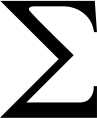
\includegraphics[width=0.225cm]{Bilder/Sigma.png} \nodepart{lower} 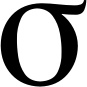
\includegraphics[width=0.225cm]{Bilder/sigma.png}};
        }
        % Draw the left input layer nodes
            \foreach \name / \xn in {1,...,\ni}{
            % This is the same as writing \foreach \name / \y in {1/1,2/2,3/3,4/4}
                \node[neuron,fontscale=15] (Il-\name) at (\xn*\neuronsep-\neuronsep,\y) {$i_{\xn}$};
                \node[above of=Il-\name, node distance=\inout cm] (Inl-\name) {};
                \draw [->,arrows={-Stealth[length=7pt]},densely dotted] (Inl-\name) edge (Il-\name);
            }
        % Draw the hidden layer node
            \foreach \name / \xn in {1,...,\nh}{
                \node[neuron,fontscale=15] (Hl-\xn) at ({(\ni-1)*\neuronsep/2-\neuronsep/2*(\nh-1)+(\xn-1)*\neuronsep},\y-\layersep) {$h_{\xn}$};
                \node[node distance=\inout cm, below of=Hl-\xn] (Hnl) {};
        % Connect every node in the inner layer with the hidden layer
            \foreach \source in {1,...,\ni}
                \draw [->,arrows={-Stealth[length=7pt]}] (Il-\source) edge (Hl-\xn);
                }
        % Draw the output layer node
            \foreach \name / \xn in {1,...,\no}{
                \node[neuron,fontscale=15] (Ol-\xn) at ({(\ni-1)*\neuronsep/2-\neuronsep/2*(\no-1)+(\xn-1)*\neuronsep},\y-2*\layersep) {$\Omega_{\xn}$};
                \node[node distance=\inout cm, below of=Ol-\xn] (Onl) {};
                \draw [->,arrows={-Stealth[length=7pt]},densely dotted] (Ol-\xn) edge (Onl);
        % Connect every node in the hidden layer with the output layer
            \foreach \source in {1,...,\nh}
                \draw [->,arrows={-Stealth[length=7pt]}] (Hl-\source) edge (Ol-\xn);
                }
        % Annotate the layers
            \ifthenelse{\ni>\nh}{
                \node[annot,right of=Il-\ni, node distance=\dlsize cm] (il) {\textbf{Eingabe- schicht}};
                \node[annot,below of=il] (hl) {\textbf{Verdeckte- schicht}};
            }{
                \node[annot,right of=Hl-\nh, node distance=\dlsize cm] (hl) {\textbf{Verdeckte- schicht}};
                \node[annot,above of=hl] (il) {\textbf{Eingabe- schicht}};
            }
                \node[annot,below of=hl] {\textbf{Ausgabe- schicht}};
        %-----------------------------------------
        %% rechtes Bild
            \tikzset{
                ident/.pic={
                \draw[semithick] (-\siz/4,-\siz/4) -- (\siz/4,\siz/4);
            }}
        % Draw the right input layer nodes
                \coordinate (tIr) at ($(il)-(Il-\ni)$);
                \coordinate (ttIr) at (tIr |- 0,0);
                \coordinate (Ir) at ($(il)+(ttIr)$);
            \foreach \name / \xn in {1,...,\ni}{
        % This is the same as writing \foreach \name / \y in {1/1,2/2,3/3,4/4}
                \node[neuron] (Ir-\name) at ($(Ir)+(\xn*\neuronsep-\neuronsep,0)$) {};
                \node[above of=Ir-\name, node distance=\inout cm] (Inr-\name) {};
                \pic at (Ir-\name) {ident};
                \draw [->,arrows={-Stealth[length=7pt]},densely dotted] (Inr-\name) edge (Ir-\name);
            }
        % Draw the right hidden layer node
            \foreach \name / \xn in {1,...,\nh}{
                \neurono[Hr-\xn]{$(Ir)+({(\ni-1)*\neuronsep/2-\neuronsep/2*(\nh-1)+(\xn-1)*\neuronsep},-\layersep)$}
                \node[node distance=\inout cm, below of=Hr-\xn] (Hnr) {};
        % Connect every node in the input layer with the hidden layer
            \foreach \source in {1,...,\ni}
                \draw [->,arrows={-Stealth[length=7pt]}] (Ir-\source) edge  (Hr-\xn);
            }            

                \node[fill=white,inner sep=1pt,fontscale=10] at ($(Hr-1)+({(\nh-1)*\neuronsep/2},\layersep*.5)$) {$\dots\,w_{i,h}\,\dots$};
        % Draw the right output layer node
            \foreach \name / \xn in {1,...,\no}{
                \neurono[Or-\xn]{$(Ir)+({(\ni-1)*\neuronsep/2-\neuronsep/2*(\no-1)+(\xn-1)*\neuronsep},-2*\layersep)$}
                \node[node distance=\inout cm, below of=Or-\xn] (Onr) {};
                \draw [->,arrows={-Stealth[length=7pt]},densely dotted] (Or-\xn) edge (Onr);
        % Connect every node in the hidden layer with the output layer
            \foreach \source in {1,...,\nh}
                \draw [->,arrows={-Stealth[length=7pt]}] (Hr-\source) edge  (Or-\xn);
            }
                \node[fill=white,inner sep=1pt,fontscale=10] at ($(Or-1)+({(\no-1)*\neuronsep/2},\layersep*.5)$) {$\dots\,w_{h,\Omega}\,\dots$};
\end{tikzpicture}
    \caption[Darstellung eines MLP]{Ein MLP mit einer verdeckten Schicht und verdeckten Neuronen $h$ auf der linken Seite. Die rechte Seite zeigt das gleiche Netzwerk mit den zugehörigen neuronalen Aufgaben und Gewichten.\,\protect\footnotemark{}}
    \label{fig:MLP}
\end{figure}



Im Unterschied zu den SLPs besitzen die Mehrschichtperceptrons zwischen der Eingabe- und Ausgabeschicht noch mindestens eine verdeckte Verarbeitungsschicht. Somit weisen sie \hbox{mindestens} zwei Ebenen an trainierbaren Gewichten auf. In \autoref{fig:MLP} ist ein MLP mit einer verdeckten Schicht dargestellt. Die zusätzliche Ebene von trainierbaren Gewichten ermöglicht eine beliebig genaue Approximation einer Funktion mit endlich vielen Unstetigkeitsstellen und ihrer ersten Ableitung. Hierdurch ist es diesem Netzwerk möglich neben der erwähnten XOR-Funktion auch komplexere Funktionen zu erlernen. Theoretisch können beliebig viele verdeckte Schichten aufgebaut werden aber wie \hbox{\citet{dkriesel07}} erläutert, reichen drei Ebenen von trainierbaren Gewichten aus, um jede beliebige Menge darstellen zu können.\,\citef[86 ff]{dkriesel07}

Um das MLP zu trainieren, gibt es das sogenannte Backpropagation-Verfahren, welches auf der Deltaregel aufbaut und zu den überwachten Lernalgorithmen zählt. Hierbei wird das Netzwerk in der Trainingsphase mit Informationen versorgt und das errechnete Ergebnis wird mit dem gewünschten Ergebnis verglichen. Die Abweichung wird anschließend genutzt, um die Gewichte ausgehend von den Ausgabe- hin zu den Eingabeneuronen anzupassen und die Abweichung zwischen den Ergebnissen zu minimieren. Ein bekanntes Problem dieses Verfahrens ist, dass bei mehreren verdeckten Schichten und einer konstanten Lernrate die Gewichte langsamer trainiert werden, je weiter sie sich von der Ausgabeschicht befinden.\,\citef[89 ff]{dkriesel07} Des Weiteren hat eine hohe Anzahl an Ausgabeneuronen ebenfalls einen negativen Einfluss auf die Lerngeschwindigkeit des Netzwerkes.\,\citef[124]{dkriesel07} Aus diesem Grund gibt es in der Literatur zahlreiche Verbesserungen, die hier nicht aufgeführt werden, da sie den Rahmen dieser Arbeit übersteigen würden. Auf das Backpropagation-Verfahren wird aber in \autoref{sec:Backpropagation} näher eingegangen. 


\subsubsection{Radiale Basisfunktionen (RBF)}
\begin{figure}[!hb]
    \centering
    %---------------------------------------------------------------
        %% RBF
        %-----------------------------------------
            %---------------------------------------------------------------
        %% RBF
        %----------------------------------------- 
        %% linkes Bild
        \begin{tikzpicture}[>=stealth', node distance=\layersep cm, shorten >=1pt]
        \def\layersep{1.8}          % vertikal distance between the layers
        \def\neuronsep{1.8}         % Horizontal distance between neurons
        \def\dlsize{2}              % distance between node and layer lable
        \def\inout{\layersep*.65}   % Size of in- and output-arrow
        \def\siz{.8}                % neuronsize
        \def\y{5}                   % Start of the most upper layer
        \def\ni{3}                  % Amount of input neurons
        \def\nh{4}                  % Amount of hidden neurons
        \def\no{2}                  % Amount of output neurons
        \tikzstyle{neuron}=[circle,draw=black,minimum size=\siz cm,inner sep=2pt]
        \tikzstyle{annot} = [text width=5em, text centered]
        \tikzset{fontscale/.style = {font={\fontsize{#1pt}{#1pt}\selectfont}}}
        \tikzset{
                ident/.pic={
                \draw[semithick] (-\siz/#1,-\siz/#1) -- (\siz/#1,\siz/#1);
            }}
        \newcommand{\neurono}[3][]{%
        \ifthenelse{\equal{#3}{0}}{%
            \node[neuron,circle split,inner sep=1pt,fontscale=6] (#1) at (#2)
                    {$\mathbf{||c\mathord{,}x||}$ \nodepart{lower}};
                    
            \node[fontscale=6] at ($(#2.lower)-(0,\siz/4)$){\textbf{Gauß}};
            }{
            \node[neuron,circle split,inner sep=1.3pt] (#1) at (#2)
                    {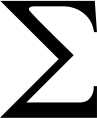
\includegraphics[width=0.225cm]{Bilder/Sigma.png} \nodepart{lower} };
            \pic at ($(#1.lower)-(0,\siz/8)$) {ident=#3};
            }}
        % Draw the left input layer nodes
            \foreach \name / \xn in {1,...,\ni}{
            % This is the same as writing \foreach \name / \y in {1/1,2/2,3/3,4/4}
                \node[neuron,fontscale=15] (Il-\name) at (\xn*\neuronsep-\neuronsep,\y) {$i_{\xn}$};
                \node[above of=Il-\name, node distance=\inout cm] (Inl-\name) {};
                \draw [->,arrows={-Stealth[length=7pt]},densely dotted] (Inl-\name) edge (Il-\name);
            }
        % Draw the hidden layer node
            \foreach \name / \xn in {1,...,\nh}{
                \node[neuron] (Hl-\xn) at ({(\ni-1)*\neuronsep/2-\neuronsep/2*(\nh-1)+(\xn-1)*\neuronsep},\y-\layersep) [fontscale=15] {$h_{\xn}$};
                \node[node distance=\inout cm, below of=Hl-\xn] (Hnl) {};
        % Connect every node in the inner layer with the hidden layer
            \foreach \source in {1,...,\ni}
                \draw [->,arrows={-Stealth[length=7pt]}] (Il-\source) edge (Hl-\xn);}
        % Draw the output layer node
            \foreach \name / \xn in {1,...,\no}{
                \node[neuron] (Ol-\xn) at ({(\ni-1)*\neuronsep/2-\neuronsep/2*(\no-1)+(\xn-1)*\neuronsep},\y-2*\layersep) [fontscale=15] {$\Omega_{\xn}$};
                \node[node distance=\inout cm, below of=Ol-\xn] (Onl) {};
                \draw [->,arrows={-Stealth[length=7pt]},densely dotted] (Ol-\xn) edge (Onl);
        % Connect every node in the hidden layer with the output layer
            \foreach \source in {1,...,\nh}
                \draw [->,arrows={-Stealth[length=7pt]}] (Hl-\source) edge (Ol-\xn);}
        % Annotate the layers
            \ifthenelse{\ni>\nh}{
                \node[annot,right of=Il-\ni, node distance=\dlsize cm] (il) {\textbf{Eingabe- schicht}};
                \node[annot,below of=il] (hl) {\textbf{Verdeckte- schicht}};
            }{
                \node[annot,right of=Hl-\nh, node distance=\dlsize cm] (hl) {\textbf{Verdeckte-/RBF- schicht}};
                \node[annot,above of=hl] (il) {\textbf{Eingabe- schicht}};
            }
                \node[annot,below of=hl] {\textbf{Ausgabe- schicht}};
        %-----------------------------------------
        %% rechtes Bild
        % Draw the right input layer nodes
                \coordinate (tIr) at ($(il)-(Il-\ni)$);
                \coordinate (ttIr) at (tIr |- 0,0);
                \coordinate (Ir) at ($(il)+(ttIr)$);
            \foreach \name / \xn in {1,...,\ni}{
        % This is the same as writing \foreach \name / \y in {1/1,2/2,3/3,4/4}
                \node[neuron] (Ir-\name) at ($(Ir)+(\xn*\neuronsep-\neuronsep,0)$) {};
                \node[above of=Ir-\name, node distance=\inout cm] (Inr-\name) {};
                \pic at (Ir-\name) {ident=4};
                \draw [->,arrows={-Stealth[length=7pt]},densely dotted] (Inr-\name) edge (Ir-\name);}
        % Draw the right hidden layer node
            \foreach \name / \xn in {1,...,\nh}{
                \neurono[Hr-\xn]{$(Ir)+({(\ni-1)*\neuronsep/2-\neuronsep/2*(\nh-1)+(\xn-1)*\neuronsep},-\layersep)$}{0}
                \node[node distance=\inout cm, below of=Hr-\xn] (Hnr) {};
        % Connect every node in the input layer with the hidden layer
            \foreach \source in {1,...,\ni}
                \draw [->,arrows={-Stealth[length=7pt]}] (Ir-\source) edge  (Hr-\xn);}
        % Draw the right output layer node
            \foreach \name / \xn in {1,...,\no}{
                \neurono[Or-\xn]{$(Ir)+({(\ni-1)*\neuronsep/2-\neuronsep/2*(\no-1)+(\xn-1)*\neuronsep},-2*\layersep)$}{6}
                \node[node distance=\inout cm, below of=Or-\xn] (Onr) {};
                \draw [->,arrows={-Stealth[length=7pt]},densely dotted] (Or-\xn) edge (Onr);
        % Connect every node in the hidden layer with the output layer
            \foreach \source in {1,...,\nh}
                \draw [->,arrows={-Stealth[length=7pt]}] (Hr-\source) edge  (Or-\xn);
            }
                \node[fill=white,inner sep=1pt,fontscale=10] at ($(Or-1)+({(\no-1)*\neuronsep/2},\layersep*.5)$) {$\dots\, w_{h,\Omega}\,\dots$};
        \end{tikzpicture}
    \caption[Darstellung eines RBF]{RBF mit drei Eingabeneuronen $i$, vier verdeckten Neuronen $h$  und zwei Ausgabeneuronen $\Omega$ auf der linken Seite. Die rechte Seite zeigt das gleiche Netzwerk mit den zugehörigen neuronalen Aufgaben und Gewichten.\,\protect\footnotemark{}}
    \label{fig:RBF}
\end{figure}
\addtocounter{footnote}{-1}     %  -1 mal die Gesamtanzahl an Fußnoten in der wrapfigure
\addtocounter{Hfootnote}{-1}    % -1 times total number of footnote(mark)s in the wrapfigure
\wrapfigfoot\footnotetext{Die linke Darstellung des RBF in \autoref{fig:RBF} wurde der Abbildung 6.1 aus \citet[111]{dkriesel07} nachempfunden.}

\gls{RBF}[s] (dargestellt in \autoref{fig:RBF}) sind Feed-Forward Netze und ähnlich wie die Perceptron-Netze schichtartig aufgebaut. Dabei besitzt jedes Neuron einer Schicht eine Verbindung zu jedem Neuron der nachfolgenden Schicht (diese Art der Verbindung zwischen den Schichten wird auch Vollverknüpfung genannt). RBFs besitzen aber genau drei Schichten und somit nur eine verdeckte Schicht. Die erste Schicht dient ebenfalls wie bei den Perceptron-Netzen nur der Verteilung der Eingabedaten an die nächste Schicht ohne jegliche Verarbeitung. Die zweite Schicht besteht aus verdeckten Neuronen, die auch als RBF-Neuronen \inlineneuron[rbf-h]{0.8} bezeichnet werden. Jedes Neuron beinhaltet eine radiale Basisfunktion als Aktivierungsfunktion. Dies sind stets positive und radialsymmetrische Funktionen. Sie besitzen ein Maximum in der Mitte (das sogenannte Zentrum~$c$) und streben gegen Null, je weiter sich die Funktion vom Mittelpunkt entfernt. Eine typische Basisfunktion ist hierbei die gaußsche Glockenkurve. Die Propagierungsfunktion bildet hier den Abstand zwischen der Eingabeinformation~$x$~und dem Zentrum~$c$~der Aktivierungsfunktion. Die Ausgabe eines RBF-Neurons gibt nun Auskunft über die Nähe der Eingabedaten zum Mittelpunkt der Basisfunktion. Schließlich sind die verdeckten Neuronen über eine gewichtete Verbindung mit den Ausgabeneuronen \inlineneuron[rbf-o]{0.8} verknüpft. Die Ausgabeneurone summieren die Ausgabe der RBF-Neuronen und geben die Summe ohne weitere Verarbeitung weiter. 

Das Training von RBFs erfolgt in zwei Schritten. Zunächst werden die Zentren der Basisfunktionen bestimmt. Dies kann zufällig erfolgen. Im nächsten Schritt werden die Gewichte zwischen der verdeckten und der Ausgabeschicht angepasst. Da nur eine Gewichtsschicht trainiert werden muss, kann hierfür die Deltaregel genutzt werden.

Ursprünglich wurden die RBFs als Interpolationsverfahren entwickelt. Daher wurde jedem Trainingsbeispiel ein Basispunkt und somit ein RBF-Neuron zugewiesen. Bei großen Datensätzen ergibt sich eine große Anzahl an verdeckten Neuronen, die einen hohen Speicherbedarf nach sich ziehen. Um mit einer geringeren Anzahl an verdeckten Neuronen auszukommen, können auch die RBF-Netze trainiert werden. Das Training der RBF-Netze findet oftmals in mehreren Stufen statt. Im ersten Schritt werden die Zentren und Formparameter durch unüberwachte Lernmethoden bestimmt. Im nächsten Schritt werden die Gewichte beispielsweise mit der Deltaregel angepasst.

Die RBFs bieten den Vorteil, dass durch das Stauchen/Strecken und Verschieben der Basisfunktionen und das anschließende Aufsummieren jede mögliche Funktion approximiert werden kann. Weiterhin wirkt sich die Anzahl an Ausgabeneuronen nicht wesentlich auf die Berechnungskomplexität aus. Im Gegenzug führt eine hohe Anzahl an Trainingsbeispielen aber auch zu einer gleich hohen Anzahl an verdeckten Neuronen und somit zu einem erhöhten Speicher- und Rechenaufwand. Eine Verringerung der Anzahl der RBF-Neuronen und anschließendes Training sind zwar möglich, bestehen aber aus mehreren Stufen und erhöhen einerseits die Algorithmuskomplexität und bieten andererseits mehr Raum für Ungenauigkeiten .\,\footnote{Vgl. \citet[73 ff]{comp_int_07}, \citet[109 ff]{dkriesel07} und \citet[261 ff]{Kroll16}.}

\subsubsection{Self Organizing Feature Maps (SOM)}
\begin{figure}[!htb]
    \centering
    %---------------------------------------------------------------
        %% SOM
        %-----------------------------------------
        %---------------------------------------------------------------
        %% SOM
        %-----------------------------------------
        %% linkes Bild
        \begin{tikzpicture}[>=stealth', node distance=\layersep cm, shorten >=1pt]
        \def\layersep{2}            % vertikal distance between the layers
        \def\neuronsep{1.5}         % Horizontal distance between neurons
        \def\dlsize{1.5}            % distance between node and layer lable
        \def\inout{\layersep*.65}   % Size of in- and output-arrow
        \def\siz{.8}                % neuronsize
        \def\y{3}                   % Start of the most upper layer
        \def\ni{5}                  % Amount of input neurons
        \def\no{3}                  % Amount of output neurons
        \tikzstyle{neuron}=[circle,draw=black,minimum size=\siz cm,inner sep=2pt]
        \tikzstyle{annot} = [text width=6em, text centered]
        \tikzset{fontscale/.style = {font={\fontsize{#1pt}{#1pt}\selectfont}}}
        \tikzset{
                ident/.pic={
                \draw[semithick] (-\siz/#1,-\siz/#1) -- (\siz/#1,\siz/#1);
            }}
        \newcommand{\neurono}[3][]{%
        \ifthenelse{\equal{#3}{0}}{%
            \node[neuron,circle split,inner sep=1pt,fontscale=6] (#1) at (#2) { $\mathbf{||c,x||}$ \nodepart{lower}};
            \node[fontscale=6] at ($(#2.lower)-(0,\siz/4)$){\textbf{Gauß}};
            }{
            \node[neuron,circle split,inner sep=1.3pt] (#1) at (#2)
                    {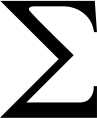
\includegraphics[width=0.225cm]{Bilder/Sigma.png} \nodepart{lower} };
            \pic at ($(#1.lower)-(0,\siz/8)$) {ident=#3};
            }}
        % Draw the left input layer nodes
            \foreach \xn in {1,...,\ni}{
                \node[neuron,fontscale=15] (Il-\xn) at (\xn*\neuronsep-\neuronsep,\y) {$i_{\xn}$};
                \node[above of=Il-\xn, node distance=\inout cm] (Inl-\xn) {};
                \draw [arrows={-Stealth[length=7pt]},densely dotted] (Inl-\xn) edge (Il-\xn);
            }
        % Draw the output layer node
            \foreach \xn in {1,...,\no}{
                \node[neuron] (Ol-\xn) at ({(\ni-1)*\neuronsep/2-\neuronsep/2*(\no-1)+(\xn-1)*\neuronsep},\y-\layersep) [fontscale=15] {$\Omega_{\xn}$};
        % Connect every node in the input layer with the output layer                
            \foreach \source in {1,...,\ni}{
                \draw [->,arrows={-Stealth[length=7pt]}] (Il-\source) edge (Ol-\xn);}}
        % Connect every node in the output layer
            \pgfmathsetmacro{\nom}{\no - 1}
            \ifthenelse{\equal{\no}{1}}{%
            }{
               \foreach \xn in {1,...,\nom}{
                    \pgfmathtruncatemacro{\xnp}{\xn + 1}
                    \draw[arrows={Stealth[length=7pt]-Stealth[length=7pt]},shorten <=1pt] (Ol-\xn) edge[bend right=45] (Ol-\xnp);
            }}
        % Annotate the layers
                \node[annot,right of=Il-\ni, node distance=\dlsize cm] (il) {\textbf{Eingabe- schicht}};
                \node[annot,below of=il] {\textbf{Ausgabe- schicht}};
        %-----------------------------------------
        %% rechtes Bild
        % Draw the right input layer nodes
                \coordinate (tIr) at ($(il)-(Il-\ni)$);
                \coordinate (ttIr) at (tIr |- 0,0);
                \coordinate (Ir) at ($(il)+(ttIr)$);
            \foreach \name / \xn in {1,...,\ni}{
        % This is the same as writing \foreach \name / \y in {1/1,2/2,3/3,4/4}
                \node[neuron] (Ir-\xn) at ($(Ir)+(\xn*\neuronsep-\neuronsep,0)$) {};
                \node[above of=Ir-\xn, node distance=\inout cm] (Inr-\xn) {};
                \pic at (Ir-\xn) {ident=4};
                \draw [->,arrows={-Stealth[length=7pt]},densely dotted] (Inr-\xn) edge (Ir-\xn);}
        % Draw the right output layer node
            \foreach \xn in {1,...,\no}{
                \neurono[Or-\xn]{$(Ir)+({(\ni-1)*\neuronsep/2-\neuronsep/2*(\no-1)+(\xn-1)*\neuronsep},-\layersep)$}{0}
                \node[node distance=\inout cm, below of=Or-\xn] (Onr) {};
                %\draw [->,arrows={-Stealth[length=7pt]},densely dotted] (Or-\xn) edge (Onr);
        % Connect every node in the hidden layer with the output layer
            \foreach \source in {1,...,\ni}
                \draw [arrows={-Stealth[length=7pt]}] (Ir-\source) edge  (Or-\xn);
            }
                \node[fill=white,inner sep=1pt,fontscale=10] at ($(Or-1)+({(\no-1)*\neuronsep/2},\layersep*.55)$) {$\dots\, w_{i,\Omega}\,\dots$};
        % Connect every node in the output layer
            \ifthenelse{\equal{\no}{1}}{%
            }{
               \foreach \xn in {1,...,\nom}{
                    \pgfmathtruncatemacro{\xnp}{\xn + 1}
                    \draw[arrows={Stealth[length=7pt]-Stealth[length=7pt]},shorten <=1pt] (Or-\xn) edge[bend right=45] (Or-\xnp);
            }}
        \end{tikzpicture}
    \caption[Darstellung eines SOM]{Eine SOM mit fünf Eingabeneuronen $i$ und drei Ausgabeneuronen $\Omega$ auf der linken Seite. Die rechte Seite zeigt das gleiche Netzwerk mit den zugehörigen neuronalen Aufgaben und Gewichten.}
    \label{fig:SOM}
\end{figure}

Die \gls{SOM}[s] (dargestellt in \autoref{fig:SOM}) wurden in den 1980ern von Teuvo Kohonen vorgestellt und werden daher in der Literatur auch als Kohonen Netzwerke bezeichnet. Die SOMs sind nah verwandt mit den RBFs. Sie bestehen aber aus zwei anstatt drei Schichten. Die Eingabeschicht dient auch der Informationsweitergabe an die Ausgabeschicht und ist mit dieser vollverknüpft. Die größte Ähnlichkeit zwischen SOM- und RBF-Netzen besteht in dem datenverarbeitenden Neuron, welches ebenfalls ein RBF-Neuron darstellt. Im Unterschied zu den RBFs liegen die Gewichte aber zwischen Eingabe- und Ausgabeschicht und es wird nur das Ausgabeneuron aktiv, das der Eingabeinformation am nächsten liegt.
Bei den SOMs ist es nun von Interesse, welches Ausgabeneuron aktiv ist und nicht, wie bei Perceptrons oder RBFs, was die Neuronen berechnen. Zusätzlich sind die Neuronen der Ausgabeschicht abhängig von der Anwendung untereinander verbunden. Durch die Art der Verbindung ergibt sich die Dimension der Ausgabe .\,\footnote{Vgl. \citet[102 ff]{Kruse15} und \citet[153 ff]{dkriesel07}.} Einige Verbindungsmöglichkeiten sind in \autoref{fig:SOM_top} dargestellt.
\begin{figure}[tb]
    \centering
        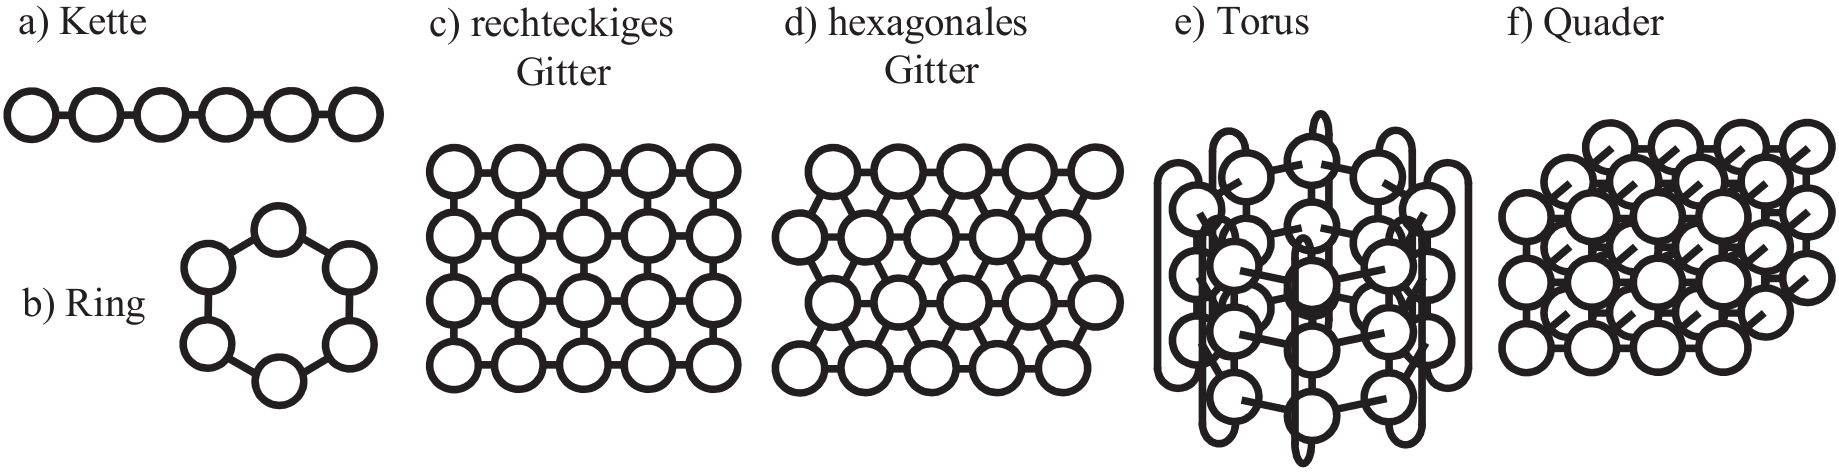
\includegraphics[width=1\textwidth]{Bilder/Netzwerke/som_top.png}
    \caption[Unterschiedliche Anordnungen der Ausgabeneuronen von SOMs]{Beispiele unterschiedlicher ein-, zwei- und dreidimensionaler Anordnungen der Ausgabeneuronen.\,\protect\footnotemark{}}
    \label{fig:SOM_top}
\end{figure}
\addtocounter{footnote}{-1}     %  -1 mal die Gesamtanzahl an Fußnoten in der wrapfigure
\addtocounter{Hfootnote}{-1}    % -1 times total number of footnote(mark)s in the wrapfigure
\wrapfigfoot\footnotetext{\autoref{fig:SOM_top} wurde aus \citet[274]{Kroll16} übernommen.}

Trainiert werden die SOMs unüberwacht, wobei die Neuronen bei der Eingabe der Testdaten um die Aktivität konkurrieren. Nach dem Prinzip \glqq the winner takes all\grqq, werden nur die Gewichte des Neurons trainiert, dessen Zentrum dem Eingabewert am nächsten liegt.\,\citef[272 ff]{Kroll16}
So können SOMs hochdimensionale Daten auf eine niedrigdimensionale Karte abbilden, wobei die Nachbarschaftsbeziehung der Daten erhalten bleibt.\,\citef[7]{Kramer09} Dies ermöglicht qualitativ die Nachbarschaftsbeziehungen zu visualisieren und Zusammenhänge von Daten durch Anhäufungen von Neuronen zu finden. Hieraus folgt, dass SOMs bei der Vorselektion von Daten eingesetzt werden können. Diese sind aber für die Approximation von Funktionen weniger geeignet.

\subsubsection{General Regression Neural Network (GRNN)}
\begin{figure}[!htb]
    \centering
    %---------------------------------------------------------------
        %% GRNN
        %-----------------------------------------
        %\includestandalone[mode=image|tex]{Bilder/Netzwerke/GRNN}
        \documentclass[tikz,border=0pt]{standalone}%
\usepackage{tikz-cd}
\usepackage{ifthen}
\usepackage{amsmath}
\usetikzlibrary{arrows,calc,intersections,shapes}
\begin{document}
%---------------------------------------------------------------
        %% GRNN
        %-----------------------------------------
        %% linkes Bild
        \begin{tikzpicture}[>=stealth', node distance=\layersep cm, shorten >=1pt]
        \def\layersep{1.8}          % vertikal distance between the layers
        \def\neuronsep{1.8}         % Horizontal distance between neurons
        \def\dlsize{2}              % distance between node and layer lable
        \def\inout{\layersep*.65}   % Size of in- and output-arrow
        \def\siz{.8}                % neuronsize
        \def\y{5}                   % Start of the most upper layer
        \def\ni{3}                  % Amount of input neurons
        \def\nh{4}                  % Amount of pattern neurons
        \def\ns{2}                  % Amount of hidden neurons
        \def\no{1}                  % Amount of output neurons
        \tikzstyle{neuron}=[circle,draw=black,minimum size=\siz cm,inner sep=2pt]
        \tikzstyle{annot} = [text width=7em, text centered]
        \tikzset{fontscale/.style = {font={\fontsize{#1pt}{#1pt}\selectfont}}}
        \tikzset{
            ident/.pic={
                \draw[semithick] (-\siz/#1,-\siz/#1) -- (\siz/#1,\siz/#1);
            }
        }
        \newcommand{\neurono}[3][]{%
            \ifthenelse{\equal{#3}{0}}{%
                \node[neuron,circle split,inner sep=.8pt,fontscale=6] (#1) at (#2)
                    { $\mathbf{||x\mathord{,}x'||}$ \nodepart{lower} };
                    
                \node[fontscale=6] at ($(#2.lower)-(0,\siz/4)$){\textbf{Exp.}};
            }{
                \ifthenelse{\equal{#3}{1}}{
                \node[neuron] (#1) at (#2) {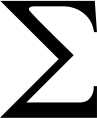
\includegraphics[width=0.3cm]{Bilder/Sigma.png}};
                }{
                \node[neuron,fontscale=15] (#1) at (#2){$\divisionsymbol$}; % if physics package is loaded use \divisionsymbol instead of \div 
                }
            }
        }
        % Draw the left input layer nodes
            \foreach \name / \xn in {1,...,\ni}{
                \node[neuron,fontscale=15] (Il-\name) at (\xn*\neuronsep-\neuronsep,\y) {$i_{\xn}$};
                \node[above of=Il-\name, node distance=\inout cm] (Inl-\name) {};
                \draw [->,arrows={-Stealth[length=7pt]},densely dotted] (Inl-\name) edge (Il-\name);
            }
        % Draw the pattern layer nodes
            \foreach \name / \xn in {1,...,\nh}{
                \node[neuron] (Hl-\xn) at ({(\ni-1)*\neuronsep/2-\neuronsep/2*(\nh-1)+(\xn-1)*\neuronsep},\y-\layersep) [fontscale=15] {$m_{\xn}$};
                \node[node distance=\inout cm, below of=Hl-\xn] (Hnl) {};
        % Connect every node in the input layer with the pattern layer
            \foreach \source in {1,...,\ni}
                \draw [->,arrows={-Stealth[length=7pt]}] (Il-\source) edge (Hl-\xn);}
        % Draw the summation layer nodes
            \foreach \name / \xn in {1,...,\ns}{
                \node[neuron] (Sl-\xn) at ({(\ni-1)*\neuronsep/2-\neuronsep/2*(\ns-1)+(\xn-1)*\neuronsep},\y-2*\layersep) [fontscale=15] {$s_{\xn}$};
                \node[node distance=\inout cm, below of=Sl-\xn] (Snl) {};
        % Connect every node in the pattern layer with the summation layer
            \foreach \source in {1,...,\nh}
                \draw [->,arrows={-Stealth[length=7pt]}] (Hl-\source) edge (Sl-\xn);}
        % Draw the output layer nodes
            \foreach \name / \xn in {1,...,\no}{
                \node[neuron] (Ol-\xn) at ({(\ni-1)*\neuronsep/2-\neuronsep/2*(\no-1)+(\xn-1)*\neuronsep},\y-3*\layersep) [fontscale=15] {$\Omega_{\xn}$};
                \node[node distance=\inout cm, below of=Ol-\xn] (Onl) {};
                \draw [->,arrows={-Stealth[length=7pt]},densely dotted] (Ol-\xn) edge (Onl);
        % Connect every node in the summation layer with the output layer
            \foreach \source in {1,...,\ns}
                \draw [->,arrows={-Stealth[length=7pt]}] (Sl-\source) edge (Ol-\xn);}
        % Annotate the layers
            \def\lni{Eingabe- schicht}                      % Lable of input layer
            \def\lnh{Musterschicht}                       % Lable of pattern layer
            \def\lns{Summierungs- schicht}                  % Lable of summation layer
            \def\lno{Ausgabe- schicht}                      % Lable of output layer
            \ifthenelse{\ni>\nh \AND \ni>\ns}{
                \node[annot,right of=Il-\ni, node distance=\dlsize cm] (il) {\textbf{\lni}};
                \node[annot,below of=il] (hl) {\textbf{\lnh}};
                \node[annot,below of=hl] (sl) {\textbf{\lns}};
            }{
                \ifthenelse{\nh>\ns}{
                    \node[annot,right of=Hl-\nh, node distance=\dlsize cm] (hl) {\textbf{\lnh}};
                    \node[annot,above of=hl] (il) {\textbf{\lni}};
                    \node[annot,below of=hl] (sl) {\textbf{\lns}};
                }{
                    \node[annot,right of=Sl-\ns, node distance=\dlsize cm] (sl) {\textbf{\lns}};
                    \node[annot,above of=sl] (hl) {\textbf{\lnh}};
                    \node[annot,above of=hl] (il) {\textbf{\lni}};
                }
                
            }
                \node[annot,below of=sl] {\textbf{\lno}};
        %-----------------------------------------
        %% rechtes Bild
        % Draw the right input layer nodes
                \coordinate (tIr) at ($(il)-(Il-\ni)$);
                \coordinate (ttIr) at (tIr |- 0,0);
                \coordinate (Ir) at ($(il)+(ttIr)$);
            \foreach \name / \xn in {1,...,\ni}{
        % This is the same as writing \foreach \name / \y in {1/1,2/2,3/3,4/4}
                \node[neuron] (Ir-\name) at ($(Ir)+(\xn*\neuronsep-\neuronsep,0)$) {};
                \node[above of=Ir-\name, node distance=\inout cm] (Inr-\name) {};
                \pic at (Ir-\name) {ident=4};
                \draw [->,arrows={-Stealth[length=7pt]},densely dotted] (Inr-\name) edge (Ir-\name);}
        % Draw the right pattern layer nodes
            \foreach \name / \xn in {1,...,\nh}{
                \neurono[Hr-\xn]{$(Ir)+({(\ni-1)*\neuronsep/2-\neuronsep/2*(\nh-1)+(\xn-1)*\neuronsep},-\layersep)$}{0}
                \node[node distance=\inout cm, below of=Hr-\xn] (Hnr) {};
        % Connect every node in the input layer with the pattern layer
                \foreach \source in {1,...,\ni}
                \draw [->,arrows={-Stealth[length=7pt]}] (Ir-\source) edge  (Hr-\xn);}
        % Draw the right summation layer nodes
            \foreach \name / \xn in {1,...,\ns}{
                \neurono[Sr-\xn]{$(Ir)+({(\ni-1)*\neuronsep/2-\neuronsep/2*(\ns-1)+(\xn-1)*\neuronsep},-2*\layersep)$}{1}
                \node[node distance=\inout cm, below of=Sr-\xn] (Snr) {};
        % Connect every node in the pattern layer with the summation layer
                \foreach \source in {1,...,\nh}
                \draw [->,arrows={-Stealth[length=7pt]}] (Hr-\source) edge  (Sr-\xn);}
            \foreach \xn in {1}{
                \foreach \source in {1,...,\nh}
                    \node[fill=white,inner sep=1pt,fontscale=10] at ($(Hr-\source)!.3+.1!(Sr-\xn)$) {$y_{\source}$};} 
        % Draw the right output layer nodes
            \foreach \name / \xn in {1,...,\no}{
                \neurono[Or-\xn]{$(Ir)+({(\ni-1)*\neuronsep/2-\neuronsep/2*(\no-1)+(\xn-1)*\neuronsep},-3*\layersep)$}{6}
                \node[node distance=\inout cm, below of=Or-\xn] (Onr) {};
                \draw [->,arrows={-Stealth[length=7pt]},densely dotted] (Or-\xn) edge (Onr);
        % Connect every node in the summation layer with the output layer
            \foreach \source in {1,...,\ns}
                \draw [->,arrows={-Stealth[length=7pt]}] (Sr-\source) edge  (Or-\xn);}
        \end{tikzpicture}
\end{document}
    \caption[Darstellung eines GRNN]{GRNN mit drei Eingabeneuronen $i$, vier Musterneuronen $m$, zwei Summierungsneuronen $s$ und einem Ausgabeneuron $\Omega$  auf der linken Seite. Die rechte Seite zeigt das gleiche Netzwerk mit den zugehörigen neuronalen Aufgaben und Gewichten.}
    \label{fig:GRNN}
\end{figure}

Vorgestellt wurde das \gls{GRNN} (dargestellt in \autoref{fig:GRNN}) von \citet{Specht1991} und ist nah verwandt mit RBF Netzen. Es zählt ebenfalls zu den Feed-Forward Netzen und besteht aus vier Schichten. Die Eingabeschicht hat dabei die Aufgabe die Eingabeinformationen an die Neuronen der Musterschicht (engl.: Pattern Layer) zu verteilen. Die nachfolgende Musterschicht besteht aus Neuronen mit einer radialen Basisfunktion als Aktivierungsfunktion. Die Ausgabe der Neuronen der Musterschicht besteht, ähnlich wie die Ausgabe der RBF-Neuronen, aus dem Abstand zwischen den Eingabedaten und den Zentren der Neuronen. Üblicherweise entspricht auch bei diesem neuronalen Netz die Anzahl der Neuronen in der Musterschicht der Anzahl an Trainingsbeispielen. Die Ausgabe der Musterschicht wird an die Summierungsschicht weitergegeben, in der die Informationen gewichtet und ungewichtet aufsummiert werden. Das Ausgangsneuron bildet einen Quotienten, bei dem die gewichtete Summe im Zähler und die ungewichtete Summe im Nenner steht.\\
Die Besonderheit dieses Netzwerkes besteht darin, dass es keinen iterativen Trainingsalgorithmus wie Backpropagation bedarf. Dies ist möglich, indem die Trainingsbeispiele als \glqq Muster\grqq~in der Musterschicht hinterlegt sind. Somit wird die den Eigabedaten zugrundeliegende Funktion durch die Trainingsbeispiele angenähert.\,\citef{Nesil2011} %\todo{Gesamtgleichung hinterlegen}\\
Der Vorteil dieses Netzwerkes liegt in der Lerngeschwindigkeit. Da die Lernbeispiele in einem Durchgang im Netzwerk gespeichert werden, werden keine mehrmaligen Gewichtsanpassungen benötigt. Hierdurch kann das Netzwerk auch nicht in einem lokalen Minimum stecken bleiben. Wie \citet{Marqueza1993} berichten, ist ein weiterer Vorteil von GRNN die geringere Beeinträchtigung bei der Regression durch verrauschte Daten im Vergleich zu Netzwerken mit Backpropagationalgorithmus.
Ein Nachteil, den RBF und GRNN teilen, ist ein größerer Bedarf an Rechenleistung mit steigender Anzahl an Trainingsbeispielen.  

\newpage

\subsubsection{Neuronale Netze von Jordan und Elman}%\\
\begin{figure}[!htb]
    \centering
    %---------------------------------------------------------------
        %% Jordannetz
        %-----------------------------------------
            %---------------------------------------------------------------
        %% Jordannetz
        %-----------------------------------------
        % trim={<left> <lower> <right> <upper>}
        \adjustbox{trim=0pt 1.9cm 0pt 0pt,clip}{
        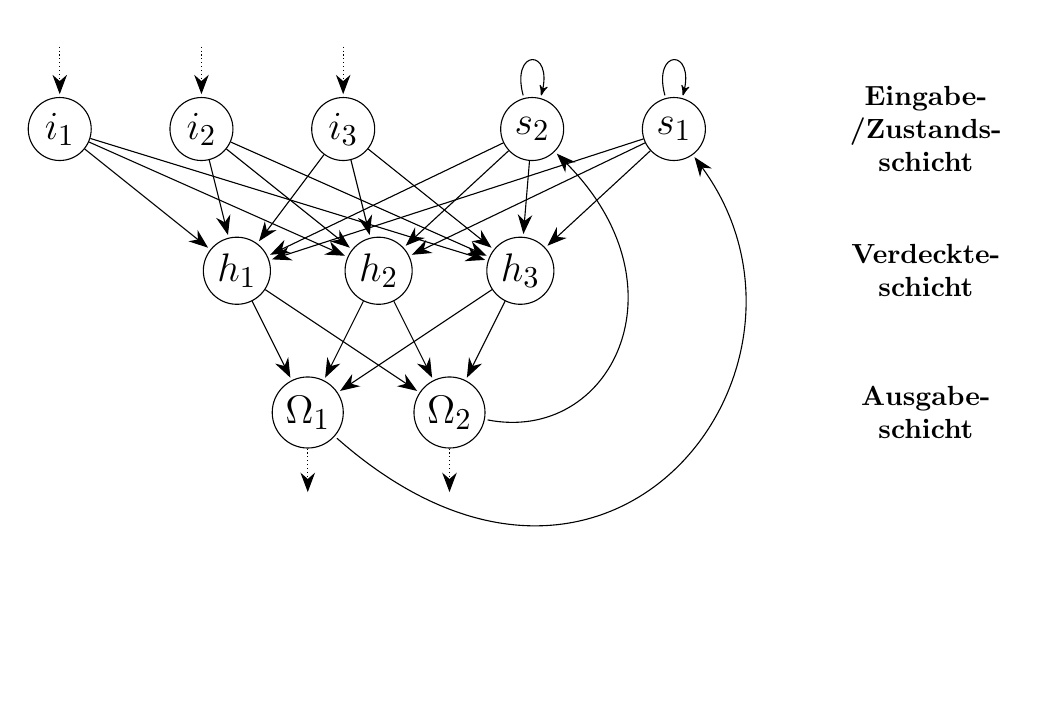
\begin{tikzpicture}[>=stealth', node distance=\layersep cm, shorten >=1pt]
        \def\layersep{1.8}            % vertikal distance between the layers
        \def\neuronsep{1.8}         % Horizontal distance between neurons
        \def\dlsize{2}            % distance between node and layer lable
        \def\inout{\layersep*.65}   % Size of in- and output-arrow
        \def\siz{.8}                % neuronsize
        \def\y{5}                   % Start of the most upper layer
        \def\ni{3}                  % Amount of input neurons
        \def\nh{3}                  % Amount of hidden neurons
        \def\no{2}                  % Amount of output neurons
        \tikzstyle{neuron}=[circle,draw=black,minimum size=\siz cm,inner sep=2pt]
        \tikzstyle{annot} = [text width=6em, text centered]
        \tikzset{fontscale/.style = {font={\fontsize{#1pt}{#1pt}\selectfont}}}
        \newcommand{\neurono}[2][]{
            \node[neuron,circle split,inner sep=2pt] (#1) at (#2)
                    {\includegraphics[width=0.225cm]{Bilder/Sigma.png} \nodepart{lower} \includegraphics[width=0.225cm]{Bilder/sigma.png}};
        }
        % Draw the input layer nodes
            \foreach \name / \xn in {1,...,\ni}{
                \node[neuron,fontscale=15] (Il-\name) at (\xn*\neuronsep-\neuronsep,\y) {$i_{\xn}$};
                \node[above of=Il-\name, node distance=\inout cm] (Inl-\name) {};
                \draw [->,arrows={-Stealth[length=7pt]},densely dotted] (Inl-\name) edge (Il-\name);
            }
        % Draw the state layer nodes
            \foreach \name / \xn in {2/1,1/2}{
                \node[neuron,fontscale=15] (Sl-\name) at (\xn*\neuronsep-\neuronsep+6,\y) {$s_{\name}$};
            }
        % Draw the hidden layer nodes
            \foreach \name / \xn in {1,...,\nh}{
                \node[neuron] (Hl-\xn) at ({(\ni-1)*\neuronsep/2-\neuronsep/2*(\nh-1)+(\xn-1)*\neuronsep+2.25},\y-\layersep) [fontscale=15] {$h_{\xn}$};
                \node[node distance=\inout cm, below of=Hl-\xn] (Hnl) {};
        % Connect every node in the input/state layer with the hidden layer
                \foreach \source in {1,...,\ni}
                    \draw [->,arrows={-Stealth[length=7pt]}] (Il-\source) edge (Hl-\xn);
             
                \foreach \source in {1,...,2}
                    \draw [->,arrows={-Stealth[length=7pt]}] (Sl-\source) edge (Hl-\xn);    
            }
        % Draw the output layer node
            \foreach \name / \xn in {1,...,\no}{
                \node[neuron] (Ol-\xn) at ({(\ni-1)*\neuronsep/2-\neuronsep/2*(\no-1)+(\xn-1)*\neuronsep+2.25},\y-2*\layersep) [fontscale=15] {$\Omega_{\xn}$};
                ,\y+2*\layersep,
                \node[node distance=\inout cm, below of=Ol-\xn] (Onl) {};
                \draw [->,arrows={-Stealth[length=7pt]},densely dotted] (Ol-\xn) edge (Onl);
        % Connect every node in the hidden/state layer with the output layer
                \foreach \source in {1,...,\nh}
                    \draw [->,arrows={-Stealth[length=7pt]}] (Hl-\source) edge (Ol-\xn);
            }
            \draw[arrows={-Stealth[length=7pt]}, shorten >=1pt, shorten <=1pt] (Ol-2) .. controls (7,1) and  (8,3) .. (Sl-2); 
            \draw[arrows={-Stealth[length=7pt]}, shorten >=1pt, shorten <=1pt] (Ol-1) .. controls (7,-2) and  (10,2) .. (Sl-1);
            \draw[arrows={-Stealth[length=7pt]}, shorten <=1pt] (Sl-1) edge[loop above] ();
            \draw[arrows={-Stealth[length=7pt]}, shorten <=1pt] (Sl-2) edge[loop above] ();
        % Annotate the layers
                \node[annot] (il) at (11,5) {\textbf{Eingabe-/Zustands- schicht}};
                \node[annot,below of=il] (hl) {\textbf{Verdeckte- schicht}};
                \node[annot,below of=hl] {\textbf{Ausgabe- schicht}};
    \end{tikzpicture}
    }
    \caption[Darstellung eines Jordannetzes]{Jordannetz mit drei Eingabeneuronen $i$, zwei Zustandsneuronen $s$, drei verdeckten Neuronen $h$ und zwei Ausgabeneuronen $\Omega$.\,\protect\footnotemark{}}
    \label{fig:Jordannetz}
\end{figure}
\addtocounter{footnote}{-1}     %  -1 mal die Gesamtanzahl an Fußnoten in der wrapfigure
\addtocounter{Hfootnote}{-1}    % -1 times total number of footnote(mark)s in the wrapfigure
\wrapfigfoot\footnotetext{\autoref{fig:Jordannetz} wurde in Anlehnung an \citet[183]{Elman1990} Figure 1 erstellt.}

Diese beiden Netzwerke ähneln sich sehr in ihrer Beschaffenheit und werden daher zusammen vorgestellt. Mehr noch stellte unter anderen die Arbeit von \citet{Jordan1986} die Grundlage für die Veröffentlichung von \citet{Elman1990} dar. Die Modelle, die in diesen Arbeiten vorgestellt werden, zählen zu den rückgekoppelten (engl.: recurrent) neuronalen Netzen. Die Grundform bildet hierbei ein Feed-Forward Netz, wie beispielsweise das MLP. Zusätzlich gibt es sogenannte Kontext bzw. Zustandsneuronen (engl.: context/state neurons). Diese bilden im übertragenden Sinne eine weitere verdeckte Schicht, da diese Schicht keine Kommunikation mit der \glqq Außenwelt\grqq~besitzt. Diese Neuronen zeichnen sich dadurch aus, dass entweder die Outputneuronen (Jordan-Netz siehe \autoref{fig:Jordannetz}) bzw. die Neuronen der verdeckten Schicht (Elamn-Netz siehe \autoref{fig:Elman}) eine Rückkopplung zu ihnen aufweisen. Zusätzlich können die Zustandsneuronen des Jordan-Netzes eine Eigenrückkopplung besitzen. %\todo{tiefer ins detail gehen}

\begin{figure}[!htb]
    \centering
    %---------------------------------------------------------------
        %% Elmannetz
        %-----------------------------------------
        %% Compiler: XeLaTeX

\documentclass[tikz,border=0pt,11pt]{standalone}%
\usepackage{tikz-cd}

\usetikzlibrary{arrows,calc,intersections,shapes}


\begin{document}
%---------------------------Elman------------------------------------------------------------------------------------------%
\begin{tikzpicture}[>=stealth', node distance=\layersep cm, shorten >=1pt]

\grid

        \def\layersep{1.8}            % vertikal distance between the layers
        \def\neuronsep{1.8}         % Horizontal distance between neurons
        \def\dlsize{2}            % distance between node and layer lable
        \def\inout{\layersep*.65}   % Size of in- and output-arrow
        \def\siz{.8}                % neuronsize
        \def\y{5}                   % Start of the most upper layer
        \def\ni{3}                  % Amount of input neurons
        \def\nh{3}                  % Amount of hidden neurons
        \def\no{2}                  % Amount of output neurons
        \tikzstyle{neuron}=[circle,draw=black,minimum size=\siz cm,inner sep=2pt]
        \tikzstyle{annot} = [text width=6em, text centered]
        \tikzset{fontscale/.style = {font={\fontsize{#1pt}{#1pt}\selectfont}}}

        \newcommand{\neurono}[2][]{
            \node[neuron,circle split,inner sep=2pt] (#1) at (#2)
                    {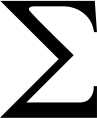
\includegraphics[width=0.225cm]{Bilder/Sigma.png} \nodepart{lower} 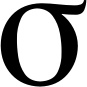
\includegraphics[width=0.225cm]{Bilder/sigma.png}};
        }
        % Draw the input layer nodes
            \foreach \name / \xn in {1,...,\ni}{
                \node[neuron,fontscale=15] (Il-\name) at (\xn*\neuronsep-\neuronsep,\y) {$i_{\xn}$};
                \node[above of=Il-\name, node distance=\inout cm] (Inl-\name) {};
                \draw [->,arrows={-Stealth[length=7pt]},densely dotted] (Inl-\name) edge (Il-\name);
            }

        % Draw the hidden layer nodes
            \foreach \name / \xn in {1,...,\nh}{
                \node[neuron] (Hl-\xn) at ({(\ni-1)*\neuronsep/2-\neuronsep/2*(\nh-1)+(\xn-1)*\neuronsep},\y-\layersep) [fontscale=15] {$h_{\xn}$};
                \node[node distance=\inout cm, below of=Hl-\xn] (Hnl) {};

        % Connect every node in the input/state layer with the hidden layer
                \foreach \source in {1,...,\ni}
                    \draw [->,arrows={-Stealth[length=7pt]}] (Il-\source) edge (Hl-\xn);
             
                %\foreach \source in {1,...,2}
                %    \draw [->,arrows={-Stealth[length=7pt]}] (Sl-\source) edge (Hl-\xn);    
            }
            
        % Draw the kontext layer nodes
            \foreach \name / \xn in {3/1,2/2,1/3}{
                \node[neuron,fontscale=15] (Sl-\name) at ($(Hl-\nh)+({\neuronsep+0.5+(\xn-1)*\neuronsep},0)$) {$k_{\name}$};
            }
            

            \draw[arrows={-Stealth[length=7pt]}, shorten >=1pt] (Hl-3) .. controls (4.3,2.2) and  (5.2,2.2) .. (Sl-3);
            \draw[arrows={-Stealth[length=7pt]}, shorten >=1pt] (Sl-3) .. controls (5.2,4.3) and  (4.3,4.3) .. (Hl-3);
            
            \draw[arrows={-Stealth[length=7pt]}, shorten >=1pt] (Hl-2) .. controls (3.5,1.8) and  (6.2,1.8) .. (Sl-2);
            \draw[arrows={-Stealth[length=7pt]}, shorten >=1pt] (Sl-2) .. controls (6.4,4.7) and  (3.3,4.7) .. (Hl-2);
            
            \draw[arrows={-Stealth[length=7pt]}, shorten >=1pt] (Hl-1) .. controls (2.4,1.5) and  (7.6,1.5) .. (Sl-1);
            \draw[arrows={-Stealth[length=7pt]}, shorten >=1pt] (Sl-1) .. controls (6.5,5)   and  (3.4,5) .. (Hl-1);

        % Draw the output layer node
            \foreach \name / \xn in {1,...,\no}{
                \node[neuron] (Ol-\xn) at ({(\ni-1)*\neuronsep/2-\neuronsep/2*(\no-1)+(\xn-1)*\neuronsep},\y-2*\layersep) [fontscale=15] {$\Omega_{\xn}$};
                ,\y+2*\layersep,
                \node[node distance=\inout cm, below of=Ol-\xn] (Onl) {};
                
                \draw [->,arrows={-Stealth[length=7pt]},densely dotted] (Ol-\xn) edge (Onl);
                
        % Connect every node in the hidden/state layer with the output layer
                \foreach \source in {1,...,\nh}
                    \draw [->,arrows={-Stealth[length=7pt]}] (Hl-\source) edge (Ol-\xn);
            }

        % Annotate the layers
                \node[annot] (il) at (12,5) {\textbf{Eingabe- schicht}};
                \node[annot,below of=il] (hl) {\textbf{Verdeckte-/Kontext- schicht}};
                \node[annot,below of=hl] {\textbf{Ausgabe- schicht}};                
 
\end{tikzpicture}
\end{document}}
    \caption[Darstellung eines Elmannetzes]{Elmannetz mit drei Eingabeneuronen $i$, drei Kontextneuronen $k$, drei verdeckten Neuronen $h$ und zwei Ausgabeneuronen $\Omega$.\,\protect\footnotemark{}}
    \label{fig:Elman}
\end{figure}
\addtocounter{footnote}{-1}     %  -1 mal die Gesamtanzahl an Fußnoten in der wrapfigure
\addtocounter{Hfootnote}{-1}    % -1 times total number of footnote(mark)s in the wrapfigure
\wrapfigfoot\footnotetext{\autoref{fig:Elman} wurde in Anlehnung an \citet[130]{dkriesel07} Abbildung 7.3 erstellt.}

Durch die zusätzliche Rückkopplung bekommt das Netzwerk ein zeitliches Gedächtnis, indem der Wert des vorherigen Durchlaufes zwischengespeichert und für die Berechnung des nächsten Wertes berücksichtigt wird. Durch die Eigenrückkopplung kann die zeitliche Ausdehnung des Gedächtnisses kontrolliert werden. 

Zum Trainieren der neuronalen Netze kann ebenfalls der Backpropagationalgorithmus angewandt werden, wobei die Eigenrückkopplungsrate während der Trainingsphase der Gewichte konstant gehalten werden muss. Hierzu wurden in der Literatur\,\citef{Pham1999} Modifikationen am Netzwerk und am Lernalgorithmus vorgestellt, um das Backpropagationverfahren auch auf die Kontextneuronen anwenden zu können.


\subsubsection{Hopfieldnetze}%\\
\begin{figure}[!htb]
    \centering
    %---------------------------------------------------------------
        %% Hopfieldnetz
        %-----------------------------------------
            %---------------------------------------------------------------
        %% Hopfieldnetz
        %-----------------------------------------
        %% linkes Bild
        \begin{tikzpicture}[ node distance=\layersep cm, shorten >=1pt]
        \def\layersep{2}            % vertikal distance between the layers
        \def\neuronsep{2}           % Horizontal distance between neurons
        \def\dlsize{2}              % distance between node and layer lable
        \def\inout{\layersep*.65}   % Size of in- and output-arrow
        \def\siz{.8}                % neuronsize
        \def\y{3}                   % Start of the most upper layer
        \def\no{3}                  % Amount of output neurons
        \tikzstyle{neuron}=[circle,draw=black,minimum size=\siz cm,inner sep=2pt]
        \tikzstyle{annot} = [text width=6em, text centered]
        \tikzset{fontscale/.style = {font={\fontsize{#1pt}{#1pt}\selectfont}}}
        \tikzset{
                ident/.pic={
                    \ifthenelse{\equal{#1}{1} \OR \equal{#1}{3}}{
                        \draw[semithick,arrows={-Latex[open]}] (0,-\siz/3) -- (0,\siz/3);
                    }{
                        \draw[semithick,arrows={Latex[open]-}] (0,-\siz/3) -- (0,\siz/3);
                    }
                    
                }
            }
        % Draw the left output layer node
            \foreach \xn in {1,...,\no}{
                \node[neuron] (Ol-\xn) at (\xn*\neuronsep-\neuronsep,\y) [fontscale=15] {$\Omega_{\xn}$};
                \node[above of=Ol-\xn, node distance=\inout cm] (Onla-\xn) {};
                \node[below of=Ol-\xn, node distance=\inout cm] (Onlb-\xn) {};
                \draw[arrows={-Stealth[length=7pt]},densely dotted] (Onla-\xn) edge (Ol-\xn);
                \draw[arrows={-Stealth[length=7pt]},densely dotted] (Ol-\xn) edge (Onlb-\xn);
            }
        % Connect every node in the output layer
            \pgfmathsetmacro{\nom}{\no - 1}
               \foreach \xn in {1,...,\nom}{
                    \pgfmathtruncatemacro{\xnp}{\xn + 1}
                    \draw[arrows={Stealth[length=7pt]-Stealth[length=7pt]},shorten <=1pt] (Ol-\xn) edge[bend right=45] (Ol-\xnp);
                        \node[fill=white,inner sep=.1pt,fontscale=10] at ($(Ol-\xnp)!.4+.1!(Ol-\xn)+(0,-0.65)$) {$w_{\xnp,\xn}$};
                }
            \draw[arrows={Stealth[length=7pt]-Stealth[length=7pt]},shorten <=1pt] (Ol-1) edge[bend right=65] (Ol-\no);
            \node[fill=white,inner sep=.1pt,fontscale=10] at ($(Ol-1)!.4+.1!(Ol-\no)+(0,-1.45)$) {$w_{1,\no}$};
        % Annotate the layers
               \node[annot,right of=Ol-\no, node distance=\dlsize cm] (ol) {\textbf{Eingabe-/Ausgabe- schicht}};
        %-----------------------------------------
        %% rechtes Bild
        % Draw the right output layer nodes
            \foreach \xn in {1,...,\no}{
                \node[neuron,right of=ol] (Or-\xn) at ($(ol)+(\xn*\neuronsep-\neuronsep,0)$) {};
                \pic at (Or-\xn) {ident=\xn};
            }
        % Draw the right upper and lower output layer nodes
            \foreach \xn in {1,...,2}{
                \node[neuron] (Orb-\xn) at ($(Or-2)+({\neuronsep/2-\neuronsep/2*(\no-1)+(\xn-1)*\neuronsep},-\layersep)$) {};
                \node[neuron] (Ora-\xn) at ($(Or-2)+({\neuronsep/2-\neuronsep/2*(\no-1)+(\xn-1)*\neuronsep},\layersep)$) {};
                \pic at (Orb-\xn) {ident=\xn};
                \pic at (Ora-\xn) {ident=\xn};
            }    
        % Connect every node in the right output layer
            \foreach \xn in {1,...,\nom}{
                \pgfmathtruncatemacro{\xnp}{\xn + 1}
                \draw[arrows={Stealth[length=7pt]-Stealth[length=7pt]},shorten <=1pt] (Or-\xn) edge (Or-\xnp);
            }    
            \foreach \xn in {1,...,\no}{
                \foreach \xp in {1,2}{
                    \draw[arrows={Stealth[length=7pt]-Stealth[length=7pt]},shorten <=1pt] (Or-\xn) edge (Ora-\xp);
                    \draw[arrows={Stealth[length=7pt]-Stealth[length=7pt]},shorten <=1pt] (Or-\xn) edge (Orb-\xp);
                }
            }
            \draw[arrows={Stealth[length=7pt]-Stealth[length=7pt]},shorten <=1pt] (Orb-1) edge[bend right=30] (Ora-2);
            \draw[arrows={Stealth[length=7pt]-Stealth[length=7pt]},shorten <=1pt] (Orb-2) edge[bend left=30] (Ora-1);
            \draw[arrows={Stealth[length=7pt]-Stealth[length=7pt]},shorten <=1pt] (Or-3)  edge[bend right=35] (Or-1);
            \node[fill=white,inner sep=1pt,fontscale=10] at ($(Or-1)+({(\no-1)*\neuronsep/2},\layersep*.5)$) {$\dots\, w_{i,j}\,\dots$};
            \node[fill=white,inner sep=1pt,fontscale=10] at ($(Or-1)+({(\no-1)*\neuronsep/2},-\layersep*.5)$) {$\dots\, w_{i,j}\,\dots$};
        \end{tikzpicture}
    \caption[Darstellung eines Hopfieldnetzes]{Hopfieldnetz mit drei Neuronen und den zugehörigen Gewichten $w$ in der Seitenansicht auf der linken Seite. Die rechte Seite zeigt das gleiche Netzwerk mit den zugehörigen neuronalen Zustand in der Draufsicht.\,\protect\footnotemark{}}
    \label{fig:Hopfield}
\end{figure}
\addtocounter{footnote}{-1}     %  -1 mal die Gesamtanzahl an Fußnoten in der wrapfigure
\addtocounter{Hfootnote}{-1}    % -1 times total number of footnote(mark)s in the wrapfigure
\wrapfigfoot\footnotetext{Die rechte Darstellung des Hopfieldnetzes in \autoref{fig:Hopfield} wurde der Abbildung 8.1 aus \citet[136]{dkriesel07} nachempfunden.}
Das Hopfield Netz (dargestellt in \autoref{fig:Hopfield}), benannt nach seinem Entwickler, zählt zu den rückgekoppelten Netzen. \citet{HOPFIELD1986} stellte ein Netzwerk vor, dass dem Verhalten von Teilchen in einem Magnetfeld nachempfunden ist.\,\citef[135]{dkriesel07} Die Neuronen dieses Netzes sind untereinander vollverknüpft, haben aber keine Verbindung zu sich selbst. Weiterhin dient die Heavisidefunktion (\autoref{fig:funktion} links) mit den möglichen Zuständen von $1$ und $-1$ als Aktivierungsfunktion und die Verbindung unter den Neuronen ist gewichtet. Die Gewichte können positiv (je höher der Wert, desto mehr tendieren die Neuronen zu gleichem Zustand), negativ (je größer der Betrag des Gewichtes, desto mehr streben die Neuronen zu unterschiedlichen Werten) oder null sein (Neuronen beeinflussen sich gegenseitig nicht). Analogiekonform kann der Zustand der Neuronen auch als Spin (Drehwinkel) der Teilchen betrachtet werden. Die Eingabe des Netzwerks geschieht durch die Festlegung der Neuronenzustände. 

Trainiert wird das Netz, indem die Trainigsbeispiele eingegeben werden und die Gewichte nach der Beziehung zueinander verändert werden. Am Ende der Trainingsphase haben die Gewichte einen hohen positiven Wert, bei denen die Neuronen oft den gleichen Zustand inne gehabt haben. Für hohe negative Gewichte gilt der umgekehrte Fall. Das Netzwerk sucht nach der Eingabe von Informationen selbstständig den energetisch niedrigsten Zustand zum betreffenden Eingabemuster. Dies geschieht unter Berücksichtigung der Gewichte und Veränderung der Spins. Hierbei wird der Zustand der Neuronen einzeln verändert, wobei das zu verändernde Neuron zufällig ausgewählt wird. Wenn die Spins sich nicht mehr ändern, ist der energetisch niedrigste Zustand erreicht. Die resultierende Spinverteilung der Neuronen ergibt dann die Ausgabe des Netzwerks. Hauptsächlich wird dieses Netzwerk zur Mustererkennung eingesetzt. Das zu erkennende Muster dient als Trainingsbeispiel und das Netzwerk ist dann in der Lage das gleiche Muster in verrauschter Form wiederzuerkennen.


\subsubsection{Adaptive Resonance Theory (ART)}%\\
\begin{figure}[!htb]
    \centering
    %---------------------------------------------------------------
        %% ART
        %-----------------------------------------
        %% Compiler: XeLaTeX

\documentclass[tikz,border=0pt]{standalone}%
\usepackage{tikz-cd}
\usetikzlibrary{arrows}

\begin{document}

%---------------------------ART-------------------------------------------------------------------------------------------%
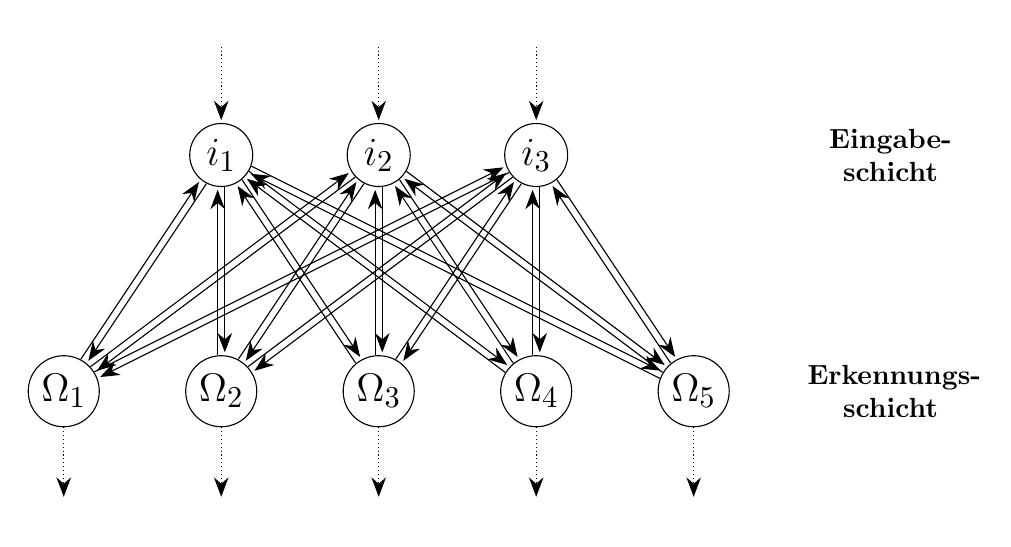
\begin{tikzpicture}[>=stealth', node distance=\layersep cm, shorten >=1pt]

        \def\layersep{3}            % vertikal distance between the layers
        \def\neuronsep{2}           % Horizontal distance between neurons
        \def\dlsize{2.5}            % distance between node and layer lable
        \def\inout{\layersep*.5}    % Size of in- and output-arrow
        \def\siz{.8}                % neuronsize
        \def\y{3}                   % Start of the most upper layer
        \def\ni{3}                  % Amount of input neurons
        \def\no{5}                  % Amount of output neurons
        \tikzstyle{neuron}=[circle,draw=black,minimum size=\siz cm,inner sep=2pt]
        \tikzstyle{annot} = [text width=6em, text centered]
        \tikzset{fontscale/.style = {font={\fontsize{#1pt}{#1pt}\selectfont}}}
        \tikzset{
            shift left/.style ={commutative diagrams/shift left={#1}},
            shift right/.style={commutative diagrams/shift right={#1}}
        }
        
        % Draw the left input layer nodes
            \foreach \xn in {1,...,\ni}{
                \node[neuron,fontscale=15] (Il-\xn) at (\xn*\neuronsep-\neuronsep,\y) {$i_{\xn}$};
                \node[above of=Il-\xn, node distance=\inout cm] (Inl-\xn) {};
                \draw [arrows={-Stealth[length=7pt]},densely dotted] (Inl-\xn) edge (Il-\xn);
            }
        % Draw the output layer node
            \foreach \xn in {1,...,\no}{
                \node[neuron] (Ol-\xn) at ({(\ni-1)*\neuronsep/2-\neuronsep/2*(\no-1)+(\xn-1)*\neuronsep},\y-\layersep) [fontscale=15] {$\Omega_{\xn}$};
                \node[node distance=\inout cm, below of=Ol-\xn] (Onl) {};
                \draw [->,arrows={-Stealth[length=7pt]},densely dotted] (Ol-\xn) edge (Onl);
        % Connect every node in the input layer with the output layer                
            \foreach \source in {1,...,\ni}{
                \draw [->,arrows={-Stealth[length=7pt]}, shift left=.3ex] (Il-\source) edge (Ol-\xn);
                \draw [->,arrows={-Stealth[length=7pt]}, shift left=.3ex] (Ol-\xn) edge (Il-\source);
                }}
                
        % Annotate the layers
                \node[annot,right of=Ol-\no, node distance=\dlsize cm] (ol) {\textbf{Erkennungs- schicht}};
                \node[annot,above of=ol] (il) {\textbf{Eingabe- schicht}};
                
        \end{tikzpicture}
\end{document}
    \caption[Darstellung eines ART]{Vereinfachte Darstellung des ART-Netzes. Mit der Eingabeschicht oben und der Erkennungsschicht unten. Die Steuerungs- und Kontrollneuronen wurde der Übersicht halber nicht dargestellt.\,\protect\footnotemark{}}
    \label{fig:ART}
\end{figure}
\addtocounter{footnote}{-1}     %  -1 mal die Gesamtanzahl an Fußnoten in der wrapfigure
\addtocounter{Hfootnote}{-1}    %  -1 times total number of footnote(mark)s in the wrapfigure
\wrapfigfoot\footnotetext{Die Darstellung des ART-Netzes in \autoref{fig:ART} wurde der Abbildung 11.1 aus \citet[174]{dkriesel07} nachempfunden.}
%\todo{Grafik Buch:Fausett-S.233}
Den Grundstein für die Theorie des \gls{ART}-Netzes (dargestellt in \autoref{fig:ART}) legte \citet{Grossberg1973} und es zählt zu den rückgekoppelten Netzen, welche unbeaufsichtigt lernen. Das ART1, das hier näher erläutert wird, wurde von \citet{Carpenter1987} vorgestellt. Dieses Netzwerk wurde mit dem Hintergedanken entwickelt, dass die bis dato vorgestellten Netzwerktypen Schwierigkeiten gehabt haben, neue Informationen zu bestehenden hinzuzufügen, ohne die bisherigen Informationen zu \glqq vergessen\grqq . Daher ist das ART Netzwerk in der Lage binäre Muster in Klassen einzuteilen, wobei es zusätzlich neue Klassen finden kann. 

Aufgebaut ist das Netzwerk aus zwei Schichten, nämlich der Eingabeschicht und der \hbox{Erkennungsschicht}, wobei die Erkennungsschicht auch für die Ausgabe der Informationen zuständig ist. Beide Schichten sind untereinander vollverknüpft. Hierbei wird der Informationsfluss von den Eingabeneuronen zu den Erkennungsneuronen hin als Bottom-Up Verbindung bezeichnet und der rückwärtige Informationsfluss als Top-Down Verbindung. Anfänglich wird das Netzwerk mit unbestimmten Gewichten initialisiert. Darauffolgend werden binäre Eingaben von der gleichnamigen Schicht an die Erkennungsschicht weitergegeben, wo nach dem Winner-Takes-All-Schema das Neuron mit der größten Aktivierung ausgewählt wird. Nun werden die Gewichte der Bottom-Up Verbindung, die zum \glqq Gewinnerneuron\grqq~führen, erhöht. Hiermit wird die Klassenzugehörigkeit des Eingabemusters verstärkt. Die Aktivität der Erkennungsschicht wird anschließend über die Top-Down Verbindung an die Eingabeschicht zurückgegeben. Hier werden ebenfalls nur die Gewichte trainiert, die vom \glqq Gewinnerneuron\grqq~zur Eingabeschicht führen. Die \glqq Aktiviät\grqq~wird so von einer Schicht an die andere und wieder zurück geleitet, wodurch der Begriff der Resonanz geprägt wird.\\
Es kommt vor, dass mehrere Neuronen der Erkennungsschicht eine gleiche Aktivität aufweisen. In diesem Fall erzeugt ein Steuerungsneuron ein zusätzliches Ausgabeneuron und ordnet diesem das aktuelle Muster zu. Bei der Eingabe ähnlicher Muster stellt sich die Frage, wann ein Neuron aktiv werden darf und wann gelernt wird. Hierfür existieren im ART-Netz Kontrollneurone, welche diese Spezialfälle durch verschiedene mathematische Regeln behandeln.\\
Der Vorteil dieses Netzes ist nicht nur, dass es die Eingabe in Klassen einordnen kann, sondern durch die Aktivierung des Ausgabeneurons auch verraten kann, wie ein typischer Vertreter dieser Klasse aussieht. Als größter Kritikpunkt gilt hier die Notwendigkeit von Spezialfallunterscheidungen, die durch diverse \glqq IF-Abfragen\grqq~abgefangen werden müssen.\,\citef[173 ff]{dkriesel07}\\
Wie zu Beginn dieses Unterkapitels durch ART1 angedeutet, gibt es nicht das ART-Netz, sondern eine Vielzahl von Weiterentwicklungen und Verbesserungen. Einige erlauben neben binären auch kontinuierliche Eingaben, andere bieten eine höhere Lerngeschwindigkeit .\,\footnote{Vgl. \citet[C2.2:1 ff]{Fiesler96} und \citet[89 ff]{Gurney1997}.} 

%Eine genauere Beschreibung und Übersicht der ART-Familie geben \citet[C2.2:1 ff]{Fiesler96} und \citet[89 ff]{Gurney1997}.

%\newpage

\subsubsection{Cascade-Correlation Netz (CCNN)}%\\
\begin{figure}[!htb]
    %\centering
    %---------------------------------------------------------------
        %% CCNN
        %-----------------------------------------
        \includestandalone[mode=image|tex,trim=0pt 0pt 0pt .8cm,clip]{Bilder/Netzwerke/CCNN}
    \caption[Darstellung eines CCNN]{Vereinfachte Darstellung des Cascade-Correlation Netzes mit den Eingabeneuronen $i$, verdeckten Neuronen $h$ und Ausgabeneuronen $\Omega$. Das Kandidatneuron trägt in dieser Darstellung die Bezeichnung $h_k$.\,\protect\footnotemark{}}
    \label{fig:ccnn}
\end{figure}
\addtocounter{footnote}{-1}     %  -1 mal die Gesamtanzahl an Fußnoten in der wrapfigure
\addtocounter{Hfootnote}{-1}    % -1 times total number of footnote(mark)s in the wrapfigure
\wrapfigfoot\footnotetext{Die \autoref{fig:ccnn} wurde der Figure 2 aus \citet[3]{Balazs2009} nachempfunden.}

Das Cascade-Correlation Modell (dargestellt in \autoref{fig:ccnn}) wurde als überwacht lernendes Feed-Foreward Netzwerk von \citet{Fahlman1990} vorgestellt. Die Idee hinter \gls{CCNN} ist, dass es zunächst mit einem SLP initialisiert und angelernt wird und solange nach Bedarf selbstständig neue Neuronen hinzufügen kann, bis der gewünschte Fehlerterm erreicht ist.\\
Genauer gesagt wird nach der Initialisierung des SLP das Netzwerk trainiert und der Fehlerterm zwischen der Ausgabe und der Lösung des Trainingsbeispiels beobachtet. Falls nicht der gewünschte Wert erreicht wird, fügt der Algorithmus ein verdecktes Neuron (das sogenannte Kandidatneuron) hinzu und trainiert dieses. Hier liegt auch der Unterschied zwischen den anderen Mehrschichtnetzen. Wird ein Kandidatneuron hinzugefügt, so werden zunächst gewichtete Verbindungen zu den bisherigen Neuronen (hierzu zählen die Eingabe- wie auch die verdeckten Neuronen) gebildet, mit Ausnahme der Ausgabeneuronen. Die Gewichte des neu erzeugten Neurons werden nun mit einem Lernalgorithmus (siehe Anhang~\ref{sec:deltaregel}) trainiert, wobei die Gewichte der anderen Neuronen eingefroren werden. Nach einem im Vorfeld festgelegten Fehlerreduktionsterm wird das Training des Kandidatneurons beendet. Als nächstes wird das Kandidatneuron mit einer gewichteten Verbindung ebenfalls mit den Ausgabeneuronen verbunden. Nun werden alle Gewichte mit Ausnahme der Gewichte der Ausgabeneuronen eingefroren und mit Hilfe eines Lernalgorithmus für einschichtige Netze (beispielsweise mit der Deltaregel) trainiert.\\
\citet{Fahlman1990} beschreiben auch die Möglichkeit, mehrere Kadidatneurone gleichzeitig zu trainieren und das Erfolgversprechendste in das Netzwerk einzubinden. Hierdurch wird die Möglichkeit reduziert in einem lokalen Minimum stecken zu bleiben. Zusätzlich können die Kandidatneuronen unterschiedliche Aktivierungsfunktionen beinhalten und das so entstehende inhomogene Netzwerk kann zu eleganteren Lösungen führen im Vergleich zu homogenen Netzwerken.\\
Der Vorteil dieses Netzwerkes besteht neben des sehr schnellen Lernvorgangs darin, dass das Netzwerk je nach Problemstellung die eigene Größe und Topologie selbst bestimmen kann. \citet{Balazs2009} gibt an, dass die CCNN aber auch leicht überangepasst (engl.: overfit) werden können.\\
%\todo{Grafik}
%\citet{Fahlman1991} stellte das rückgekoppeles Cascade-Correlation Netz (RCC) vor. Dieses Netzwerk (dargestellt in \farbig{Abbildung ??}) ist inspiriert durch das Elamn Netz. Aber anstatt Verbindungen zu Neuronen vorherigen Schichten zu bilden, welches das CCNN Konzept verletzen würde, besitzen die verdeckten Neuronen und die Kandidatneurone eine gewichtete Eigenrückkopplung. Mit dieser Änderung ist das Netz in der Lage, neben den Eigenschaften des CCNN, Muster in Zeitdiskreten Daten zu erkennen. Wie aber \citet{Kirschninga1995} feststellen hat die Grundform des RCC probleme große Gruppen von Mustern mit unterschiedlichen Eigenschaften zu erkennen. Bei einer großen Datenlage scheint das Netzwerk sogar zuvor gelernte Muster zu vergessen.  

%\newpage
\subsection{Gegenüberstellung der Netzwerke}
In diesem Unterabschnitt werden zunächst die Anwendungsgebiete künstlicher neuronaler Netze kategorisiert. Anschließend werden die vorgestellten Netzwerke vor dem Hintergrund der Charakterisierung in \autoref{sec:char} und der Anwendungsgebiete tabellarisch gegenübergestellt. Unter Berücksichtigung von \citet{Fiesler96} können die Anwendungsgebiete von neuronalen Netzen in folgende Kategorien eingeteilt werden.
\begin{itemize}
\item[\textbf{$\bullet$}] \textbf{Klassifizierung}\\%
Klassifizierung beschreibt das Zusammenfassen von Einheiten in vordefinierte Gruppen anhand ihrer Eigenschaften.
\citet{Fiesler96} unterscheiden unter den Klassifizierern zwei Paradigmen:
    \begin{itemize}
    \item[\textbf{$\circ$}] \textit{Nächster Nachbar}:\\%
    In dem Ansatz des nächsten Nachbarns (engl.: nearest neighbor) erfolgt die Klassifizierung eines unbekannten Musters anhand der Bewertung seiner Ähnlichkeit mit einigen Referenzmustern (den sogenannten Prototypen) jeder Klasse. Das unbekannte Muster wird der Klasse zugewiesen, die einem Prototypen am nächsten liegt/ähnelt.
    
    \item[\textbf{$\circ$}] \textit{Regression}:\\%
    Bei der Klassifizierung durch Regression wird versucht, eine Klasse anhand eines Musters vorherzusagen, indem der Fehlerterm zwischen den Eingabe- und Zielmustern minimiert wird.
    \end{itemize}


\item[\textbf{$\bullet$}] \textbf{Kombinatorische Optimierung}\\%
Die kombinatorische Optimierung beinhaltet die Suche nach einer \glqq optimalen\grqq~Lösung für ein Problem unter einer großen Menge an möglichen Lösungen. 
 

\item[\textbf{$\bullet$}] \textbf{Assoziatives Gedächtnis}\\%
Allgemein betrachtet, ist das assoziative Gedächtnis (engl.: associative memorie) ein Speichersystem, welches erlaubt ein Datenelement einem anderen zuzuordnen. Somit ermöglicht der Zugriff auf eines der Elemente den Zugriff auf das andere.
Die Assoziation kann dabei, wie in dem nachfolgend genannten Beispiel eins-zu-eins, eins-zu-viele oder viele-zu-viele erfolgen.
In Hinblick auf künstliche neuronale Netze wird das assoziative Gedächtnis unterschieden in:
    \begin{itemize}
    \item[\textbf{$\circ$}] \textit{Autoassoziativ}:\\%
    Beim autoassoziativem Gedächtnis ist die Ausgabe ähnlich oder gleich der \hbox{Eingabe}. Wird beispielsweise das Bild eines Hauses im Gedächtnis \glqq hinterlegt\grqq , ruft die Eingabe eines Fensters das Bild des gesamten Hauses ab.
    
    \item[\textbf{$\circ$}] \textit{Heteroassoziativ}:\\%
    Hier unterscheidet sich die Ausgabe von der Eingabe. Wird das Bild eines Fensters eingegeben kann als Ausgabe das Wort \glqq Fenster\grqq~erfolgen.\,\citef[F1.2 ff]{Fiesler96}
    
    \end{itemize}

\end{itemize}

Die genannten Kategorien sind aber nicht als starr und klar umgrenzt anzusehen. Besonders die Beschreibung des assoziativen Gedächtnisses kann ebenfalls als Klassifizierungen angesehen werden. \citet{Gurney1997} weist auf die schmale bis fließende Abgrenzung der Begrifflichkeiten hin. Hier kann das Verhältnis der Anzahl von Eingabe- zu Ausgabeneuronen darüber entscheiden, ob ein Netzwerk als Klassifizierer oder assoziatives Gedächtnis angesehen wird. Ist die Anzahl an Eingabeneuronen groß im Vergleich zu der Anzahl an Ausgabeneuronen, so wird das Netzwerk oft als Klassifizierer bezeichnet. Unterscheidet sich die Anzahl zwischen Eingabe- und Ausgabeneuronen nur geringfügig oder gar nicht, so tendiert man das Netzwerk als assoziatives Gedächtnis zu beschreiben.\,\citef[117 f]{Gurney1997} In der Literatur werden explizit Verfahren beschrieben, wie ein klassifizierungsfähiges Netzwerk als assoziatives Gedächtnis eingesetzt werden kann.\,\citef[F1.4:3 ff]{Fiesler96}

%In diesem Abschnitt erfolgt eine Zusammenfassung der Eigenschaften der vorgestellten Modelle.



\begin{filecontents*}{modelle.tex}
{\setstretch{1.0}
\captionsetup{skip=1pt,margin=5pt,position=below} %skip=1pt,
\rowcolors{3}{tableShade}{white}

\begin{longtable}{llZZ}
    \caption{Gegenüberstellung vorgestellter Modelle} \label{tab:ann_modell}\\
    \toprule
    \hiderowcolors

        Modell          & Neuronale Verbindung           & Lernverfahren     & Anwendung           \\
    \midrule
    \endfirsthead
        \multicolumn{4}{c}{\footnotesize \tablename\ \thetable{}: Fortsetzung der vorherigen Seite} \\
    \toprule
        %\multicolumn{1}{l}{\textbf{Verweis}} & \multicolumn{1}{Z}{\textbf{Modell}} & \multicolumn{1}{Z}{\textbf{Lernalgorithmus}} & \multicolumn{1}{Z}{\textbf{Markt}} & \multicolumn{1}{Z}{\textbf{Performancemaß}} \\
        Modell          & Neuronale Verbindung           & Lernverfahren     & Anwendung           \\

    \midrule
    \endhead
    \midrule
        \multicolumn{4}{c}{{\footnotesize \tablename\ \thetable{}: Fortsetzung auf der nächsten Seite}} \\
    \bottomrule
    \endfoot
    \bottomrule
        \caption*{\footnotesize K-r/nn:Klassifikation durch Regression/nächster-Nachbar, AM-h/a:Assoziatives Gedächtnis durch Heteroassoziation/Autoassoziation, KO:Kombinatorische Optimierung }
        
    \endlastfoot
    \showrowcolors
        MLP             & Feed-Forward                  & überwacht         & K-r, AM-h, AM-a                       \\
        RBF             & Feed-Forward                  & überwacht         & K-nn\,\protect\footnotemark{}, AM-h   \\
        SOM             & Recurren-lateral              & unüberwacht       & K-nn, KO, AM-h                        \\
        GRNN            & Feed-Forward                  & unüberwacht       & K-r                                   \\
        Jordan/Elman    & Recurren-indirekt             & überwacht         & K-r, AM-h                             \\
        Hopfield        & Recurren-vollverknüpft        & unüberwacht       & AM-a, KO                              \\
        ART             & Recurren-vollverknüpft        & unüberwacht       & K-nn, AM-h                            \\
        CCNN            & Feed-Forward                  & überwacht         & K-r, AM-h                             \\
        %RCC             & R-d       & überwacht         & K-r, AM-h                             \\
        
\end{longtable}

}
\end{filecontents*}
\LTXtable{\textwidth}{modelle}
\addtocounter{footnote}{-1}     %  -1 mal die Gesamtanzahl an Fußnoten in der wrapfigure
\addtocounter{Hfootnote}{-1}    % -1 times total number of footnote(mark)s in the wrapfigure
\wrapfigfoot\footnotetext{Vgl. \citet[F1.2:4]{Fiesler96}.}


In \autoref{tab:ann_modell} werden nun die in diesem Abschnitt gesammelten Informationen zusammengefasst. In der ersten Spalte werden die vorgestellten Netzwerkmodelle genannt. Nachfolgend ist die Charakteristik der Topologie des entsprechenden Netzwerkes aufgeführt. Gefolgt von dem üblicherweise angewandtem Lernverfahren und abschließend werden die möglichen Anwendungskategorien des Netzwerkes genannt. Dabei werden die Anwendungen aus Gründen der besseren Übersicht abgekürzt und am Ende der Tabelle voll ausgeschrieben.